% DAC Paper
\documentclass{sig-alternate}
\usepackage{subfigure}

\pagestyle{empty}
\frenchspacing
%
\begin{document}
\conferenceinfo{DAC'07,}{June 4 -8, 2007, San Diego, California, USA.}
\CopyrightYear{2007}
\crdata{978-1-59593-638-7/07/0004}
% Do not want to print date
\date{}
\toappear{
This paper is based on research funded in part by UCLA CENS, NSF
under award 0520006, U.S. ONR under award N000140610253, U.S. ARL and the
U.K. MoD under Agreement W911NF-06-3-0002.
Any opinions expressed
in this paper are  those of the authors and do not necessarily reflect the views
of the funding agencies.
\the\boilerplate\par
{\confname{\the\conf}} \the\confinfo\par \the\copyrightetc.}


\title{A System For Coarse Grained Memory Protection In Tiny Embedded Processors}

\author{Ram Kumar, Akhilesh Singhania, Eddie Kohler, Mani Srivastava}
\author{
\alignauthor Ram Kumar, Akhilesh Singhania, Andrew Castner, Eddie Kohler, Mani Srivastava \\
	\affaddr{University of California at Los Angeles}\\
	\affaddr{420 Westwood Plaza, Los Angeles, CA, USA}\\
	\email{\{ram,akhi,mbs\}@ee.ucla.edu, \{castner,kohler\}@cs.ucla.edu}
}

\maketitle
\thispagestyle{empty}


\begin{abstract}
%%%%%%%%%%%%%%%%%
% ABSTRACT
%%%%%%%%%%%%%%%%% 
\noindent
Many sensor nodes contain resource constrained microcontrollers where user
level applications, operating system components, and device drivers share
a single address space with no form of hardware memory protection.
%
Programming errors in one application can easily corrupt the state of
the operating system or other applications.
%
In this thesis, we propose \textit{Harbor}, a memory protection system that
prevents many forms of memory corruption.
%
We use fault isolation (``sandboxing'') to restrict application memory
accesses and control flow to protection domains within the address
space.
%
%Limited memory on sensor nodes precludes static partitioning of the
% address space into different domains.
%
A flexible and efficient \emph{memory map} data structure records
ownership and layout information for memory regions; writes are
validated using the memory map.
%
Control flow integrity is preserved by maintaining a \emph{safe stack}
that stores return addresses in a protected memory region.
%
Run-time checks validate computed control flow instructions.
%
Cross domain calls perform low-overhead control transfers between domains.
%
Checks are introduced by rewriting an application's compiled
binary. 
%
The sandboxed result is verified on the sensor node before it is admitted
for execution. 
%
Harbor's fault isolation properties depend only on the
correctness of this verifier and the Harbor runtime.
%
%Sensor nodes only need to trust the correctness of the verifier in
% the overall system.
%
We have implemented and tested Harbor on the SOS operating system.
%
Harbor detected and prevented memory corruption caused by programming
errors  in application modules that had been in use for several
months.
%
Harbor's overhead, though high, is less than that of application-specific
virtual machines, and reasonable for typical sensor workloads.

We partition the Harbor protection primitives into hardware and
software components to design a Micro Memory Protection Unit (UMPU)
for resource constrained embedded processors.
%
The hardware-software co-design approach offers the benefits of protection with a
minimal performance impact.
%
UMPU's area overhead is modest and can be easily accommodated without
increasing the die area of a chip.
%
UMPU extensions require no modifications to the instruction set of the embedded
processor thereby making it usable with the existing toolchains; a very
practical feature of the design.

\end{abstract}
%

\vspace{1mm}
\noindent
{\bf Categories and Subject Descriptors:} C.3 {[Special - \\Purpose and Application-Based Systems]}: {Real-time and embedded systems}

\vspace{1mm}
\noindent
{\bf General Terms:} Performance, Design, Reliability

\vspace{1mm}
\noindent
{\bf Keywords:} Memory Protection, Software Fault Isolation

%===============================================
% INTRODUCTION
%===============================================
\section{Introduction}
\label{sec:intro}
%
This document describes the design and implementation of the Micro Memory Protection Unit (uMPU).
%
For the motivation and architectural principles, refer to the uMPU research paper.
%
An overview of our system highlighting all its components is shown in Figure~\ref{fig:sys_overview}.
%
The final firmware image is composed of multiple software modules that need to be protected from one another.
%
%The software components are installed in separate protection domains.
%
A cross domain linking mechanism (described in Section~\ref{sec:cross_domain_linking}) installs the software modules in separate protection domains.
%
The cross domain linker generates a software jump table that assists the processor in determining the identity of the currently active domain.
%
The Memory Map (described in Section~\ref{sec:memmap}) tracks layout and ownership information for the protected address space.
%
The firmware image interacting with the memory map and hardware enhanced run-time checkers is guaranteed to be memory safe.
%
The detailed description of the architectural extensions is given in Section~\ref{sec:archext}.
%
\begin{figure}[htbp]
   \centering
   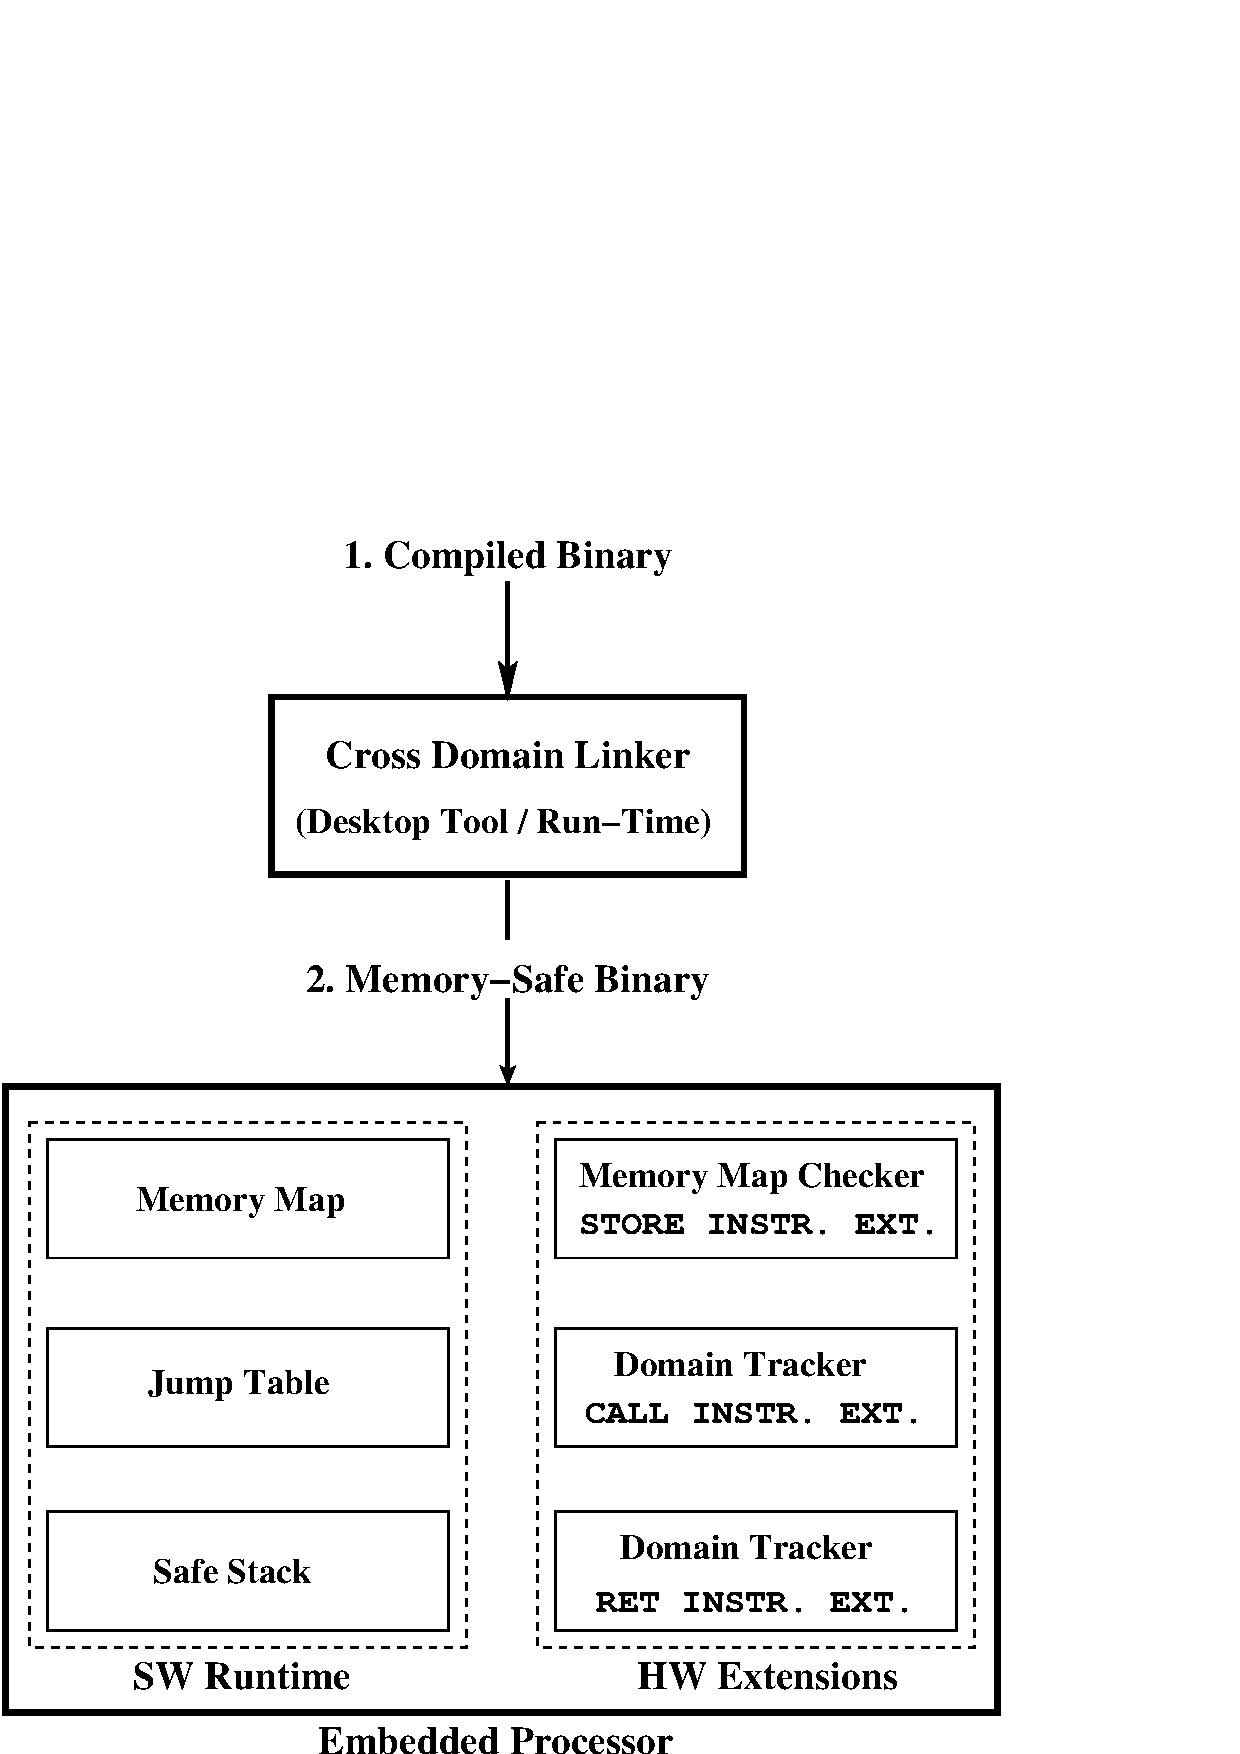
\includegraphics[height = 2.0in, keepaspectratio=true]{figures/sysoverview.pdf} 
   \caption{System Overview}
   \label{fig:sys_overview}
\end{figure}
%

%===========================================================
% MEMORY MAP SECTION
%===========================================================
\section{Memory Map Manager}
\label{sec:memmap}
%
Creating and enforcing protection domains is a challenging task on
resource constrained embedded platforms.
%
Initial SFI designs allowed a sandboxed module to access a single
contiguous range of memory~\cite{wahbe93sfi}.
%
Motes' limited physical memory and absence
of virtual memory precludes this partitioning; such a partition would
constrain applications by severely limiting available memory and lead
to internal fragmentation, extremely wasteful on severely resource
constrained platforms.
%
%% Static contiguous partitioning is only possible in desktop systems
%% with large address spaces~\cite{wahbe93sfi}.
%
Harbor's \emph{memory map} abstraction was designed with the following
requirements:
%
first, it should have a small and customizable memory footprint;
%
second, it should permit arbitrary layout of state within the data memory;
%
and third, it should be easy to incorporate into existing
operating systems.
%
We propose a design that satisfies these requirements.
%
%-----------------------------------------------------------------
\subsection{Data Structure}
%
We assume a sensor node's address space is partitioned by the operating
system into small, contiguous \emph{blocks} of equal size, then allocated
to domains in \textit{segments} consisting of sets of contiguous blocks.
%
(On AVR, SOS's block size is 8~bytes.)
%
The allocation of segments to domains could be static (at compile
time) or dynamic (through malloc).
%
A domain could be allocated multiple segments that are scattered
randomly across entire address space.
%
The Harbor memory map contains \emph{per-block} access permissions for
the entire address space.
%
The main operation of the memory map is to store and retrieve access
permissions for a given address.
%
Its design goal is to balance lookup efficiency and the extra storage
required for the permissions table.
%
The memory map contains ownership information (a domain identity) for every
block of memory, and encodes information about memory layout, such as
the start of a logical allocation segment.
%
The memory map must contain sufficient permission bits per block to encode
the total number of domains supported by the system.
%
Supporting two distinct domains (kernel and user) requires just one
domain bit per block, four domains require two domain bits per block,
and so forth.
%
Table~\ref{tab:mmap_table} shows an example of Harbor's memory map encoding
in a system with 8 domains.
%
\begin{table}[htdp]
\centering
\small{
\begin{tabular}{|c|l|}
	\hline
	Code & Meaning\\
	\hline
	1111 & Free, or start of kernel allocated segment\\
	1110 & Later portion of kernel allocated segment\\
	xxx1 & Start of user allocated segment\\
	xxx0 & Later portion of user allocated segment\\
	\hline
\end{tabular}}
\caption{Memory map information encoding for 8-domain protection.}
\label{tab:mmap_table}
\end{table}

%
The memory map is a configurable data structure; tradeoffs between
the inter-module protection and memory map size are discussed in
Section~\ref{sec:mmapdesignspace}.
%
%The design of memory map uses two bits of encoded information per
%block to provide memory protection.
%
%Due to the severe memory resource constraints, the memory map is
%designed to have a very small memory footprint. 
%
%The memory map is organized as a byte array where each byte is packed
%to store permission information about multiple blocks.
%
%Such an organization was chosen for maximum storage efficiency and
%minimum resource utilization.
%
%The memory protection mechanism intercepts every write operation of a
%user module to ensure that the permissions are not violated.
%
%The main task of the memory map manager is to store or retrieve the
%permissions for any given address.
%
%--------------------------------
\subsubsection{Address Translation}
\label{sec:memtrans}
%
Figure~\ref{fig:addr_memmap_translate} shows how an address is looked up in
the memory map.
%
Assuming a block size of 8 bytes, the last three bits of address are an
offset into a given block.
%
The remaining bits of the address represent a block number in data memory.
%
Access permissions are packed into a byte.
%
If encoded information is stored in four bits (for 8-domain
protection), then each byte would contain information for two
contiguous memory blocks.
%
Therefore, the last bit of block number selects a memory map record
from within an access permissions byte.
%
The remaining bits of the block number form an index into the memory map table.
%
This design was chosen to minimize memory footprint.
%
\begin{figure}[htbp]
  \centering
  \includegraphics[height=2.0in,
  keepaspectratio=true]{figures/memaddrtrans.eps}
  \caption{Address to memory map translation (8-domain mode)}
  \label{fig:addr_memmap_translate}
\end{figure}
%
%------------------------------
\subsubsection{Memory Map API}
%
The memory map data structure and address translation operations are
encapsulated in an object accessible through the API
in Table~\ref{tab:memmap_api}. 	
%
%
% If we optimize the memory map table to not include certain portions
% of the address space, then what will happen if we accidentally pass
% an unmapped address ?
%
%
%
\begin{table}[htdp]
   \centering
   \small{
   \begin{tabular}{|l|}
   \hline
   Prototype and Description \\
   \hline
   \texttt{int8\_t memmap\_set(uint8\_t blkID, uint8\_t nBlks, uint8\_t
   domID)}\\
   Set owner of segment [BlkID, BlkID + nBlks) to domID \\
   \hline
   \texttt{uint8\_t memmap\_get(uint8\_t blkID)}\\
   Get owner and layout of block number BlkID \\
   \hline
   \end{tabular}
   }
   \centering
   \caption{Memory map API}
   \label{tab:memmap_api}
\end{table}
%
%
%========================================================================================================================================
% MEMORY MAP CHECKER
%========================================================================================================================================
\subsection{Memory Map Checker}
\label{sec:mmapchecker}
%
Harbor's run-time checks validate memory accesses, in particular writes.
%
These accesses are validated using a protection model.
%
Our memory map checker enforces the protection model described earlier:
each user module can write only into its own domain.
%
% Further, a single trusted domain in the system is allowed to access all memory.
%
The memory map checker belongs to the trusted domain.
%
%A run-time checker restricts the memory access of user modules to permissible regions.
%
%The access control permissions are stored and tracked by the memory map manager.
%
%The policy used for access control can vary.
%
%The most common policy is to prevent the user modules from ever writing to a memory region that is owned by the kernel.
%
%The modules are instrumented to introduce checks before every write operation that needs protection.
%
%   // Get permissions through bit shifts
%   // uint8_t perms_bm = (BLOCK_TYPE_BM << ((mmap_offset >> 3) << 1));
Pseudocode for a write access check in a system with 8-domain protection is shown in Figure~\ref{fig:checker}.
%
\begin{figure} [htbp]
  \centering
  \begin{tiny}
\begin{verbatim}
write_access_check(addr_t addr, data_t data) {
   // Check is for writes outside stack region
   if (addr < STACK_PTR) {
      // Address translation: Get table index
      uint16_t blk_num = (addr >> log2_blk_size);
      uint16_t mmap_index = (blk_num >> log2_rec_per_byte);
      // Retrieve memory map byte
      uint8_t mmap_byte = MEM_MAP_PERMS_TBL[mmap_index];
  
      // Get the appropriate record in byte
      if (blk_num & SWAP_MASK) swap(mmap_byte);
      uint8_t mmap_owner = mmap_byte & OWNER_MASK;
      uint8_t first_blk_in_segment = mmap_byte & 1;

      // Validate access
      if (mmap_owner != curr_dom_id
          || (first_blk_in_segment && addr points to block metadata))
         mem_access_exception();

      // Perform store
      st addr, data;
   } else {
      // Check for writes to stack 
      stack_access_check(addr, data);
   } 
}
\end{verbatim}
      \end{tiny}
  \vskip-\baselineskip
  \caption{Pseudocode for Memory Map Checker (8-domain protection)}
  \label{fig:checker}
\end{figure}
%

The write access checker performs three operations.
%
First, it performs address translation to retrieve the byte containing
ownership information from the memory map table for a given address.
%
Second, it locates the appropriate record within that byte and determines
the domain of the block's owner.
%generates a bit mask from the address offset to derive the actual permission.
%
Third, it compares this domain ID and the current executing user module's domain ID.
%
A store is allowed only if these domains match.
%
As mentioned previously, the memory map manager does not maintain
permissions for run-time stack;
%
write accesses to the run-time stack are subject to a different
check described in Section~\ref{subsec:stackguard}.
%

%
\begin{figure}[htpb]
 \centering
  \mbox{
    \subfigure[Memory map byte for two
    domains]{\label{fig:memmaptwodoms}\includegraphics[width=2in,
      keepaspectratio = true]{figures/memmaptwodoms.eps}}
    \hspace{0.2in}
    \subfigure[Bit-Mask Lookup
    Table]{\label{fig:perm_lut}\includegraphics[height=1.5in,
      keepaspectratio = true]{Figures/perms_lut_opt.eps}}
  }
  \caption{Memory Map Checker Optimizations (2-domains)}
\end{figure}   
%
% \begin{figure}[htbp]
%   \centering
%    \includegraphics[height=1in, keepaspectratio=true]{figures/perms_lut_opt.jpg} 
%    \caption{Lookup table optimization to implement bit-shift operations}
%    \label{fig:perm_lut}
% \end{figure}
%
%-----------------------------------------
\subsubsection{Bit-Mask Lookup Table}
\label{sec:bitmasklut}
%
Next we discuss a few implementation details in the design of
memory map.
%
The memory map checker described in Figure~\ref{fig:checker} is
designed for 8 protection domains.
%
The checker operation can be further optimized for a system with only 2
protection domains.
%
In a 2 domain system, the \texttt{curr\_dom\_id} is always going to be
the untrusted domain; because the checks are introduced only in the
untrusted domain.
%
Hence a store is valid if the memory block belongs to the untrusted
domain.
%
A memory map record for 2-domain protection requires only 2 bits.
%
Therefore, 4 memory map records can be efficiently packed into a byte
as shown in Figure~\ref{fig:memmaptwodoms}.
%
The bit-mask required to retrieve the correct memory map record is
generated through complex bit shift operations as shown in
Figure~\ref{fig:perm_lut}.
%
The operation takes 32 clock cycles on ATMEGA128L as there is no
instruction level support for arbitrary bit shifts.
%
Therefore, we use a lookup table stored in flash memory to retrieve
the bit-masks.
%
Organization of the lookup table and its operation is described in
Figure~\ref{fig:perm_lut}.
%
The table lookup takes only 8 clock cycles.
%
%--------------------------------------------------
\subsubsection{Memory Heap Metadata}
%
%% This section describes a practical issue that is faced while using
%% memory map with heaps used for dynamic memory allocation.
%
An implementation detail involves the protection of heap metadata, such as
the owner and/or size an allocated segment.
%
SOS stores this metadata in the segment itself as shown in
Figure~\ref{fig:sos_free_list}.
%
This complicates the write access check, since heap metadata is
effectively kernel-domain information and must be protected from wild
writes.
%
%% This is unlike desktop systems where each process has its own heap.
%
%% Heap implementations store metadata information in data-structures
%% that are embedded within allocated memory.
%
%For example, SOS kernel implements ownership tracking of memory
%segments.
%
%During module unloading, kernel uses the ownership information to
%free all memory owned by that module.
%
Since the SOS kernel stores this metadata in a segment's first
memory block, %% as shown in Figure~\ref{fig:sos_free_list}.
%
%% This organization enables the heap to efficiently reclaim memory that
%% is freed.
%
%The segment size information is used to implement the dynamic memory
%allocate and free routines.
%
%% However, modules can overwrite the metadata, as it lies within the block
%% boundary.
%% %
%% Recall that permissions are stored only at block granularity.
%
the memory map checker protects the metadata in
the first block of any segment from user writes.
%
The memory map table's layout information supports this check by
identifying the starting block of any segment.
%
The metadata checks are also implemented using the lookup table for
improved efficiency.
%
\begin{figure} [h]
  \centering
    {\tiny
\begin{verbatim}
typedef struct _Block {
   uint16_t segmentSize;
   union {
      uint8_t userPart[BLOCK_SIZE - sizeof(uint16_t)];
      struct {
         struct _Block *prev;
         struct _Block *next;
      };
   };
} Block;
\end{verbatim} }
\caption{SOS block metadata}
\label{fig:sos_free_list}
\end{figure}
%
%Checks are introduced by a re-write of binary generated by cross-compiler tool-chain.
%
%We describe design of binary rewriter in Section~\ref{sec:writeverify}
%
%The CIL (C Intermediate Language)~\cite{cil02necula} framework catches all the writes made by the user module and inserts the appropriate write access check.
%
%In future, the checks would be introduced by an automatic binary re-write of the user modules.
%
%The binary re-writes would be performed at the load time of the
%modules into the sensor network.
%========================================================================================================================================
% MEMORY MAP FOR PROTECTION
%========================================================================================================================================
\subsection{Using the Memory Map for Protection}
\label{sec:mmap_for_protection}
%
Information stored in the memory map can be used for a variety of protection models;
%
our protection model restricts programs from writing to memory outside their domain.
%
%% We discuss how memory map can be used in any system to enforce this protection model.
%


%
Systems using a memory map need to ensure the following four conditions.
%
First, the memory map should accurately reflect the current ownership and
layout of memory.
%
In any real system, memory is constantly allocated, freed, and/or
transferred from one module to another.
%
The memory map should be immediately updated when any of these events
occur; thus, SOS's
%
\texttt{malloc}, \texttt{free}, and
\texttt{change\_own} system calls were modified to update the memory
map data structure. 
%
Second, only the block owner should be permitted to free or change its ownership.
%
This condition is necessary as one module may accidentally (due to
programming errors) attempt to free memory being used by other
modules.
%
%% It prevents a module from accidentally hijacking memory that is
%% owned by other modules.
%
To enforce this condition, the system needs to track the currently
active domain (Section~\ref{sec:cfmgr}).
%
%
Third, direct access to the memory map API (described in Table~\ref{tab:memmap_api})
should be restricted to trusted domains, such as the kernel.
%
%% If modules are allowed direct access to memory map API, then we can no
%% longer trust information stored in it.
%% %
%% Programming bugs can cause incorrect parameters to be passed to memory map API.
%% %
%% In SOS, kernel is treated as a trusted domain and is allowed access to memory map API.
%
%% User modules are prevented access by restricting their control flow.
%
In addition, the blocks storing memory map data structures should be owned
by a trusted domain, preventing
%
accidental corruption of the memory map data structure.
%


%The memory map manager tracks the permission information for every block in the address space of the sensor node.
%
A memory map can be easily incorporated into software systems.
%
As an example, we describe how SOS's memory map provides multi-domain protection.
%
%Memory map Two domain protection in SOS is easily implemented.
%
The memory map is initialized such that all statically allocated kernel
memory blocks are marked as owned by kernel.
%
%% Statically allocated blocks are used exclusively by kernel only and
%% user modules never read or write to them.
%
The remaining portion of the address space is partitioned into a heap,
a safe stack (further described in Section~\ref{subsec:safe_stack}), and a run-time stack.
%
The heap is divided into blocks, so the minimum granularity of 
%%  and a set of contiguous blocks (segments)
%% are dynamically allocated to user modules or the kernel upon request.
%
memory allocation is a block.
%
% Mention something about the choice of block size
%
The heap's memory map is initially marked as free.
%
The safe stack is marked as belonging to the kernel domain.
%
The run-time stack has no memory map;
%
we discuss run-time stack protection in Section~\ref{subsec:stackguard}.
%
Our implementation modified 150 lines of code, about 1\% of the 12720-line
SOS kernel; the change was
%
mostly localized to
dynamic memory management routines. 
%
%
% What are the implications of over-writing the stack ?
%
%The memory map manager works closely with the dynamic memory manager in the SOS operating system.
%
%Any request for dynamic memory is passed to the memory map manager that sets the correct permissions for the set of allocated blocks.
%
%During free operation, the memory map manager automatically clears the permissions.
%
%The dynamic memory manager in SOS permits the ownership change for dynamically allocated memory blocks.
%
%The memory map manager tracks any changes to the permissions that are caused due to the ownership transfer of a set of memory blocks.
%
%
%
%The dynamic memory allocator in SOS maintains a free list of unused memory blocks.
%
%Figure~\ref{fig:sos_free_list} shows the data structure implementing a memory block in SOS kernel.
%
%The data structure contains metadata that stores the number of contiguous blocks constituting the current segment.
%
%This information is critical for the correct functioning of the dynamic memory allocator.
%
%However, as the metadata is a part of the memory block, it can be easily corrupted by the user module.
%
%This is because the protection is provided only at the block level granularity.
%
%The problem was solved by eliminating the metadata information from
%the block structure and deriving it at run-time based upon the layout
%information stored in the memory map table.
%
%The absence of the metadata impacts the execution overhead of the dynamic memory operations.
%
%xs
%--------------------------------------------------------------------------------
\subsection{Design Tradeoffs}
\label{sec:mmapdesignspace}
Harbor provides a number of design knobs that allow systems to trade
off protection and resource utilization.
%
First, the memory map data structure is configured by changing the
number of bits stored per block to match the number of domains
required by a system.
%
For example, four bits per block support up to eight protection
domains.
%
We have found eight domains to be sufficient for most sensor network
systems using SOS.
%
Two bits per block can create a two-domain system (a user/kernel
model).
%
Increasing the number of bits stored per block increases the size of
the memory map.
%
%We have currently evaluated scenarios with only one SOS module per
%domain.
%
%However, Harbor does not pose this restriction.
%
%Systems have freedom to group a set of modules and assign them to a
%single domain.
%
%The block size can be set based upon typical size of memory objects
%used in the system.
%

Second, there is a tradeoff between the size of the memory map and the
amount of memory fragmentation.
%
Larger block size leads to increased internal fragmentation, but
reduces the number of blocks and thereby the size of the memory map.
%
For example, a block size of 256 bytes is suitable for the large image
and matrix objects passed around in the Cyclops
imager~\cite{cyclops05sensys}.
%
Mica2 based modules use a block size of 8 bytes.
%
Harbor and SOS currently support a single fixed block size for the
entire heap; an extension might permit using different block
granularity in different memory regions.
%

Third, the memory map can be configured to track ownership and layout
in only a subset of the entire address space, reducing its space
overhead. 
%
%This reduces the size of memory map required for protection.
%
For example, in SOS the memory map tracks only the heap and safe
stack.
%
%Memory accesses made by user modules to addresses outside the heap
%(except those into run-time stack) are considered invalid.
%
%% This reduces the size of memory map by 33\% (See
%% Table~\ref{tab:kernel_size_comparison})
%
In general, the size of the memory map can be reduced by decreasing
the fraction of memory reserved for the heap.
% as opposed to run-time stack.
%
%Many software systems create custom heap implementations
%(e.g. Message pools in SNACK~\cite{ben04snack}) that cover only a
%fraction of total address space.
%






% %
% Creating and enforcing protection domains is a challenging task on resource constrained embedded platforms.
% %
% Limited memory prohibits static contiguous partitioning of address space into multiple domains.
% %
% Such a contiguous partition would introduce design constraints on applications by limiting memory that is available to them.
% %
% Static contiguous partitioning is only possible in desktop systems with large address spaces~\cite{wahbe93sfi}
% %
% We designed protection domains with following requirements.
% %
% First, small and customizable memory footprint.
% %
% Second, no design constraints for user applications.
% %
% Third, easy to incorporate into existing systems.
% %
% Memory map data structure satisfies these requirements.
% %
% %
% %
% %
% %========================================================================================================================================
% % MEMORY MAP DATA STRUCTURE
% %========================================================================================================================================
% \section{Data Structure}
% %
% Address space of sensor node processor is partitioned into blocks of equal sizes.
% %
% \textit{Block} is a small contiguous region of memory.
% %
% Memory is allocated to domains as \textit{segments}; a set of contiguous blocks.
% %
% Allocation of segments to domains could be static (at compile time) or dynamic (through malloc).
% %
% A domain could be allocated multiple segments that are scattered randomly across entire address space.
% %
% \textit{Memory map contains access permissions for every block of address space.}
% %
% Main operation of memory map is to to store and retrieve access permissions for a given address.
% %
% The goal in design of memory map it to balance efficiency of lookup with extra storage required for table.
% %
% Memory map specifies two pieces of information.
% % 
% First, it contains ownership information (domain identity) for every block of memory.
% %
% Second, it encodes information about memory layout such as start of a logical segment of allocation to programs.
% %
% An example of actual encoded information and their meaning is specified in Table~\ref{tab:mmap_table}.
% %
% \begin{table}[htdp]
% \centering
% \small{
% \begin{tabular}{|c|l|}
% 	\hline
% 	Code & Meaning\\
% 	\hline
% 	1111 & Free or Start of Kernel Allocated Segment\\
% 	1110 & Later portion of Kernel Allocated Segment\\
% 	xxx1 & Start of User (0 - 6) Allocated Segment \\
% 	xxx0 & Later portion of User (0 - 6) Allocated Segment\\
% 	\hline
% \end{tabular}}
% \caption{Encoded information in memory map table for multi-domain protection}
% \label{tab:mmap_table}
% \end{table}

% %
% %The design of memory map uses two bits of encoded information per block to provide memory protection.
% %
% %Due to the severe memory resource constraints, the memory map is designed to have a very small memory footprint. 
% %
% %The memory map is organized as a byte array where each byte is packed to store permission information about multiple blocks.
% %
% %Such an organization was chosen for maximum storage efficiency and minimum resource utilization.
% %
% %The memory protection mechanism intercepts every write operation of a user module to ensure that the permissions are not violated.
% %
% %
% %
% %
% %The main task of the memory map manager is to store or retrieve the permissions for any given address.
% %
% Mapping from the address to the memory map is shown in Figure~\ref{fig:addr_memmap_translate}.
% %
% Assuming block size of 8 bytes\footnote{Our implementation on AVR uses block size of 8 bytes}, last three bits of address are offset into a given block.
% %
% Remaining bits represent block number in data memory.
% %
% Permissions are packed into a byte.
% %
% If encoded information is stored in two bits (for two-domain protection), then each byte would contain information of four contiguous memory blocks.
% %
% Therefore, last two bits of block number represent byte offset of permission.
% %
% Remaining bits index into memory map table.
% %
% This particular design of memory map table was chosen to minimize memory footprint.
% %
% Memory map is a configurable data-structure and the tradeoffs between the level of protection and the size of memory map is discussed in Section~\ref{sec:designspace}.
% %
% Memory map data structure and address translation operations are encapsulated into an object that is accessible through an API described in Table~\ref{tab:memmap_api}. 	
% %
% %
% \begin{figure}[htbp]
%    \centering
%    \includegraphics[height=2.5in, keepaspectratio=true]{figures/memaddrtrans.eps} 
%    \caption{Address to memory map translation (Two Domain Mode)}
%    \label{fig:addr_memmap_translate}
% \end{figure}
% %
% % If we optimize the memory map table to not include certain portions of the address space, then what will happen if we accidentally pass an unmapped address ?
% %
% %
% %
% \begin{table}[htdp]
%    \centering
%    \small{
%    \begin{tabular}{|l|l|}
%    \hline
%    Prototype & Description \\
%    \hline
%    int8\_t memmap\_set(uint8\_t blkID, uint8\_t nBlks,& Set owner of segment\\
%    uint8\_t domID) & [BlkID, BlkID + nBlks) to domID \\
%    \hline
%    uint8\_t memmap\_get(uint8\_t blkID) & Get owner and layout\\
%    & of block number BlkID \\
%    \hline
%    \end{tabular}
%    }
%    \centering
%    \caption{Memory Map API}
%    \label{tab:memmap_api}
% \end{table}
% %
% %
% %========================================================================================================================================
% % MEMORY MAP FOR PROTECTION
% %========================================================================================================================================
% \section{Using Memory Map For Protection}
% \label{subsec:mmap_for_protection}
% %
% Information stored in memory map data-structure can be used for creating a variety of protection models;
% %
% our protection model restricts programs from writing to memory outside their domain.
% %
% We discuss how memory map can be used in any system to enforce this protection model.
% %



% %
% Systems using memory map need to ensure following four conditions.
% %
% First, memory map should accurately reflect current ownership and layout.
% %
% In any real system, memory is constantly allocated, de-allocated or transferred from one module to another.
% %
% Memory map should be immediately updated when any of these events occur.
% %
% For example in SOS, \texttt{malloc}, \texttt{free} and \texttt{change\_own} system calls were modified to update memory map data structure. 
% %
% Second, only block owner should be permitted to free or change its ownership.
% %
% This condition is necessary as one module may accidentally (due to programming errors) free up memory that is being used by other module in the system.
% %
% Also it prevents a module from accidentally hijacking memory that is owned by other modules.
% %
% To enforce this condition, system needs to track the current active domain.
% %
% We describe implementation details of tracking current active application in Section~\ref{sec:cfmgr}.
% %
% Third, access to memory map API (described in Table ~\ref{tab:memmap_api}), should be restricted to single trusted domain.
% %
% If modules are allowed direct access to memory map API, then we can no longer trust information stored in it.
% %
% Programming bugs can cause incorrect parameters to be passed to memory map API.
% %
% In SOS, kernel is treated as a trusted domain and is allowed access to memory map API.
% %
% User modules are prevented access by restricting their control flow.
% %
% Fourth, blocks storing memory map data structure should be owned by the trusted domain.
% %
% This condition prevents accidental corruption of memory map data structure.
% %


% %The memory map manager tracks the permission information for every block in the address space of the sensor node.
% %
% Memory map can be easily incorporated into software systems.
% %
% As an example, we describe usage of memory map in SOS operating system to provide two domain (User-Kernel) protection.
% %
% %Memory map Two domain protection in SOS is easily implemented.
% %
% Memory map is initialized such that all statically allocated kernel memory blocks in address space are marked as owned by kernel.
% %
% Statically allocated blocks are used exclusively by kernel only and user modules never read or write to them.
% %
% Remaining portion of address space is partitioned into heap and a stack.
% %
% Heap is divided into blocks and a set of contiguous blocks (segments) are dynamically allocated to user modules or the kernel upon request.
% %
% Hence, minimum granularity of memory allocation is a block.
% %
% % Mention something about the choice of block size
% %
% Memory map for heap is initially marked as Free.
% %
% Stack has no memory map.
% %
% We discuss stack protection in Section~\ref{subsec:stackguard}.
% %
% Our implementation modified only 150 lines of code out of 12720 lines in SOS kernel.
% %
% This represents about 1\% change and most of it is localized to dynamic memory management routines. 
% %
% %
% % What are the implications of over-writing the stack ?


% %
% %The memory map manager works closely with the dynamic memory manager in the SOS operating system.
% %
% %Any request for dynamic memory is passed to the memory map manager that sets the correct permissions for the set of allocated blocks.
% %
% %During free operation, the memory map manager automatically clears the permissions.
% %
% %The dynamic memory manager in SOS permits the ownership change for dynamically allocated memory blocks.
% %
% %The memory map manager tracks any changes to the permissions that are caused due to the ownership transfer of a set of memory blocks.
% %
% %
% %
% %The dynamic memory allocator in SOS maintains a free list of unused memory blocks.
% %
% %Figure~\ref{fig:sos_free_list} shows the data structure implementing a memory block in SOS kernel.
% %
% %The data structure contains meta-data that stores the number of contiguous blocks constituting the current segment.
% %
% %This information is critical for the correct functioning of the dynamic memory allocator.
% %
% %However, as the meta-data is a part of the memory block, it can be easily corrupted by the user module.
% %
% %This is because the protection is provided only at the block level granularity.
% %
% %The problem was solved by eliminating the meta-data information from the block structure and deriving it at run-time based upon the layout information stored in the memory map table.
% %
% %The absence of the meta-data impacts the execution overhead of the dynamic memory operations.
% %
% %
% %========================================================================================================================================
% % MEMORY MAP CHECKER
% %========================================================================================================================================
% \section{Memory Map Checker}
% %
% A run-time checker is required to validate memory accesses made by software components.
% %
% Memory accesses need to be validated against a protection model.
% %
% Our memory map checker enforces the protection model that we described earlier; programs can write only into their domain.
% %
% Further, a single trusted domain in the system is allowed to access all memory.
% %
% Memory map checker belongs to the trusted domain.
% %
% %A run-time checker restricts the memory access of user modules to permissible regions.
% %
% %The access control permissions are stored and tracked by the memory map manager.
% %
% %The policy used for access control can vary.
% %
% %The most common policy is to prevent the user modules from ever writing to a memory region that is owned by the kernel.
% %
% %The modules are instrumented to introduce checks before every write operation that needs protection.
% %
% %   // Get permissions through bit shifts
%  %  // uint8_t perms_bm = (BLOCK_TYPE_BM << ((mmap_offset >> 3) << 1));
% Pseudo-code for write access checks is shown in Figure~\ref{fig:checker}.
% %
% \begin{figure} [h]
%   \centering
%     {\small
% \begin{verbatim}
% WRITE_ACCESS_CHECK(addr_t addr){
%   // Check is for writes outside stack region
%   if (addr < STACK_PTR){
  
%    // Retrieve permissions byte
%    uint16_t  mmap_index = (addr >> 5);
%    uint8_t   perms = MEM_MAP_PERMS_TBL[mmap_index];
  
%    // Generate bit mask
%    uint8_t   mmap_offset = (addr & 0x1f);
%    // Get permissions through look-up table
%    uint8_t   perms_bm = MEM_MAP_BM_LUT[mmap_offset];
   
%    // Check validity
%    if  !(perms & perms_bm) mem_access_exception();
%   } 
%  // Check for writes to stack 
%  else{
%    stack_access_check(addr);
%  } 
% }
% \end{verbatim} }
%   \caption{Pseudo-code for memory map checker (For two-domain protection)}
%   \label{fig:checker}
% \end{figure}

% %
% The write access checker performs three operations.
% %
% First, it retrieves the byte containing ownership information from memory map table for a given address.
% %
% Second, it generates a bit mask from the address offset to derive the actual permission.
% %
% Third, it checks the permission and signals memory access violation for invalid operations.
% %
% Algorithm to retrieve the permissions byte from memory map has already been discussed in Figure~\ref{fig:addr_memmap_translate}.
% %
% Generation of the bit mask requires complex bit shift operations.
% %
% These operations require 32 clock cycles on Atmega128L as there is no instruction level support for arbitrary bit shifts.
% %
% Therefore, a lookup table is used; this is stored in flash memory to minimize RAM usage.
% %
% Organization of the lookup table and its operation is described in Figure~\ref{fig:perm_lut}.
% %
% The lookup table takes only 8 clock cycles.
% %
% Therefore, the checker is designed to introduce minimal execution overhead.
% %
% The sub-routine is optimized for specific processor architecture to maximize efficiency.
% %
% %For example, the micro-controller architecture such as the Atmega128L does not have instruction level support for arbitrary bit shifts.
% %
% %
% As mentioned previously, the memory map manager does not maintain permissions for run-time stack.
% %
% Therefore, all write accesses to the stack are subject to a different check that will be discussed later.
% %
% % \begin{figure}[htbp]
% %   \centering
% %    \includegraphics[height=2.5in, keepaspectratio=true]{figures/perms_lut_opt.jpg} 
% %    \caption{Lookup table optimization to implement bit-shit operations}
% %    \label{fig:perm_lut}
% % \end{figure}
% %
% %========================================================================================================================================
% % MEMORY HEAP META-DATA
% %========================================================================================================================================
% \section{Memory Heap Meta-data}
% %
% This section describes a practical issue that is faced while using memory map with heaps used for dynamic memory allocation.
% %
% Applications running on embedded micro-controllers share a single heap.
% %
% This is unlike desktop systems where each process has its own heap.
% %
% Heap implementations store meta-data information in data-structures that are embedded within allocated memory.
% %
% %For example, SOS kernel implements ownership tracking of memory segments.
% %
% %During module unloading, kernel uses the ownership information to free all memory owned by that module.
% %
% For example, SOS kernel stores segment size as meta-data within first memory block of segment as shown in Figure~\ref{fig:sos_free_list}.
% %
% This organization enables the heap to efficiently reclaim memory that is freed.
% %
% %The segment size information is used to implement the dynamic memory allocate and free routines.
% %
% However, modules can overwrite the meta-data as it lies within block boundary.
% %
% Recall, that permissions are stored only at block granularity.
% %
% Therefore, memory map checker is modified such that the meta-data in the first block of any segment is protected from writes.
% %
% Note that memory map table maintains layout information that identifies the starting block of any segment.
% %
% Additional checks are also implemented using look-up table for improved efficiency.
% %
% \begin{figure} [h]
%   \centering
%     {\small
% \begin{verbatim}
% typedef struct _Block
% {
%   uint16_t segmentSize;
%   union
%   {
%     uint8_t userPart[BLOCK_SIZE - sizeof(uint16_t)];
%     struct 
%     {
%       struct _Block *prev;
%       struct _Block *next;
%     };
%   } ;
% } Block;
% \end{verbatim} }
% \caption{Block implementation in SOS kernel}
% \label{fig:sos_free_list}
% \end{figure}


% %
% %Checks are introduced by a re-write of binary generated by cross-compiler tool-chain.
% %
% %We describe design of binary rewriter in Section~\ref{sec:writeverify}
% %
% %The CIL (C Intermediate Language)~\cite{cil02necula} framework catches all the writes made by the user module and inserts the appropriate write access check.
% %
% %In future, the checks would be introduced by an automatic binary re-write of the user modules.
% %
% %The binary re-writes would be performed at the load time of the modules into the sensor network.

















%==============================================================================================
% CONTROL FLOW MANAGER
%==============================================================================================
\section{Control Flow Manager}
\label{sec:cross_domain_linking}
%
Programming errors can cause a module to corrupt its own state.
%
Protection domains created and enforced by the memory map manager cannot prevent such internal memory corruption.
%
Control flow within a system can be affected by internal memory corruption.
%
For example, function pointers (commonly used to implement callbacks) are stored in RAM.
%
Return addresses to function call-sites are stored in the stack.
%
Corruption of these values can cause the processor to execute arbitrary code belonging to the trusted domain.
%
%This violates one of the requirements of using memory map for protection; restricting memory map access to single trusted domain (Refer Section~\ref{subsec:mmap_for_protection}).
%
The Control Flow Manager ensures that control can never flow out of a domain except via calls to functions exported by other domains and via returns to calls from other domains.
%
Conversely, control flow can enter a domain only through an exported function or through the return site of a call that is made to a function exported by some other domain.
%
In addition, the identity of the current domain (that is executing) also needs to be tracked.
%
This information is required by the memory map checker to validate write accesses.
%
%We have implemented a Cross Domain Linking mechanism that is used to transfer control safely from caller to callee domain and vice versa.
%
%A corresponding Cross Domain Return mechanism restores control back to caller domain. 
%
Control flow integrity within a domain is preserved through the safe stack that stores return addresses.
%
%==============================================================================================
% CROSS DOMAIN LINKING
%==============================================================================================
\subsection{Cross Domain Linking}
%
A module loaded in a domain exports a set of functions that can be validly called by modules in other domains.
%
%Cross domain linking enables a module belonging to a domain to call functions in other domain.
%
%Modules in a domain are linked with modules in other domains at load-time.
%
A linker parses the set of functions exported by a domain and writes them to a \textit{jump table} in flash memory.
%
The jump table is similar in design to the processor interrupt vector table.
%
Each entry in the jump table is an instruction to jump to a valid exported function.
%
Each domain has its own jump table that contains all functions that it exports. 
%
Modules are not allowed to directly write to flash memory and therefore the jump table cannot be corrupted.
%
Modules that subscribe to functions exported by a particular domain are re-directed through the jump table of that domain.
%
This is illustrated in Figure~\ref{fig:cross_domain_call}.
%
The jump table mechanism is independent of the process used for dynamic linking i.e. exporting and subscribing to functions.
%
Linking could be done statically or dynamically on the embedded processor~\cite{dunkels06linking}.
%
\begin{figure}[htbp]
   \centering
   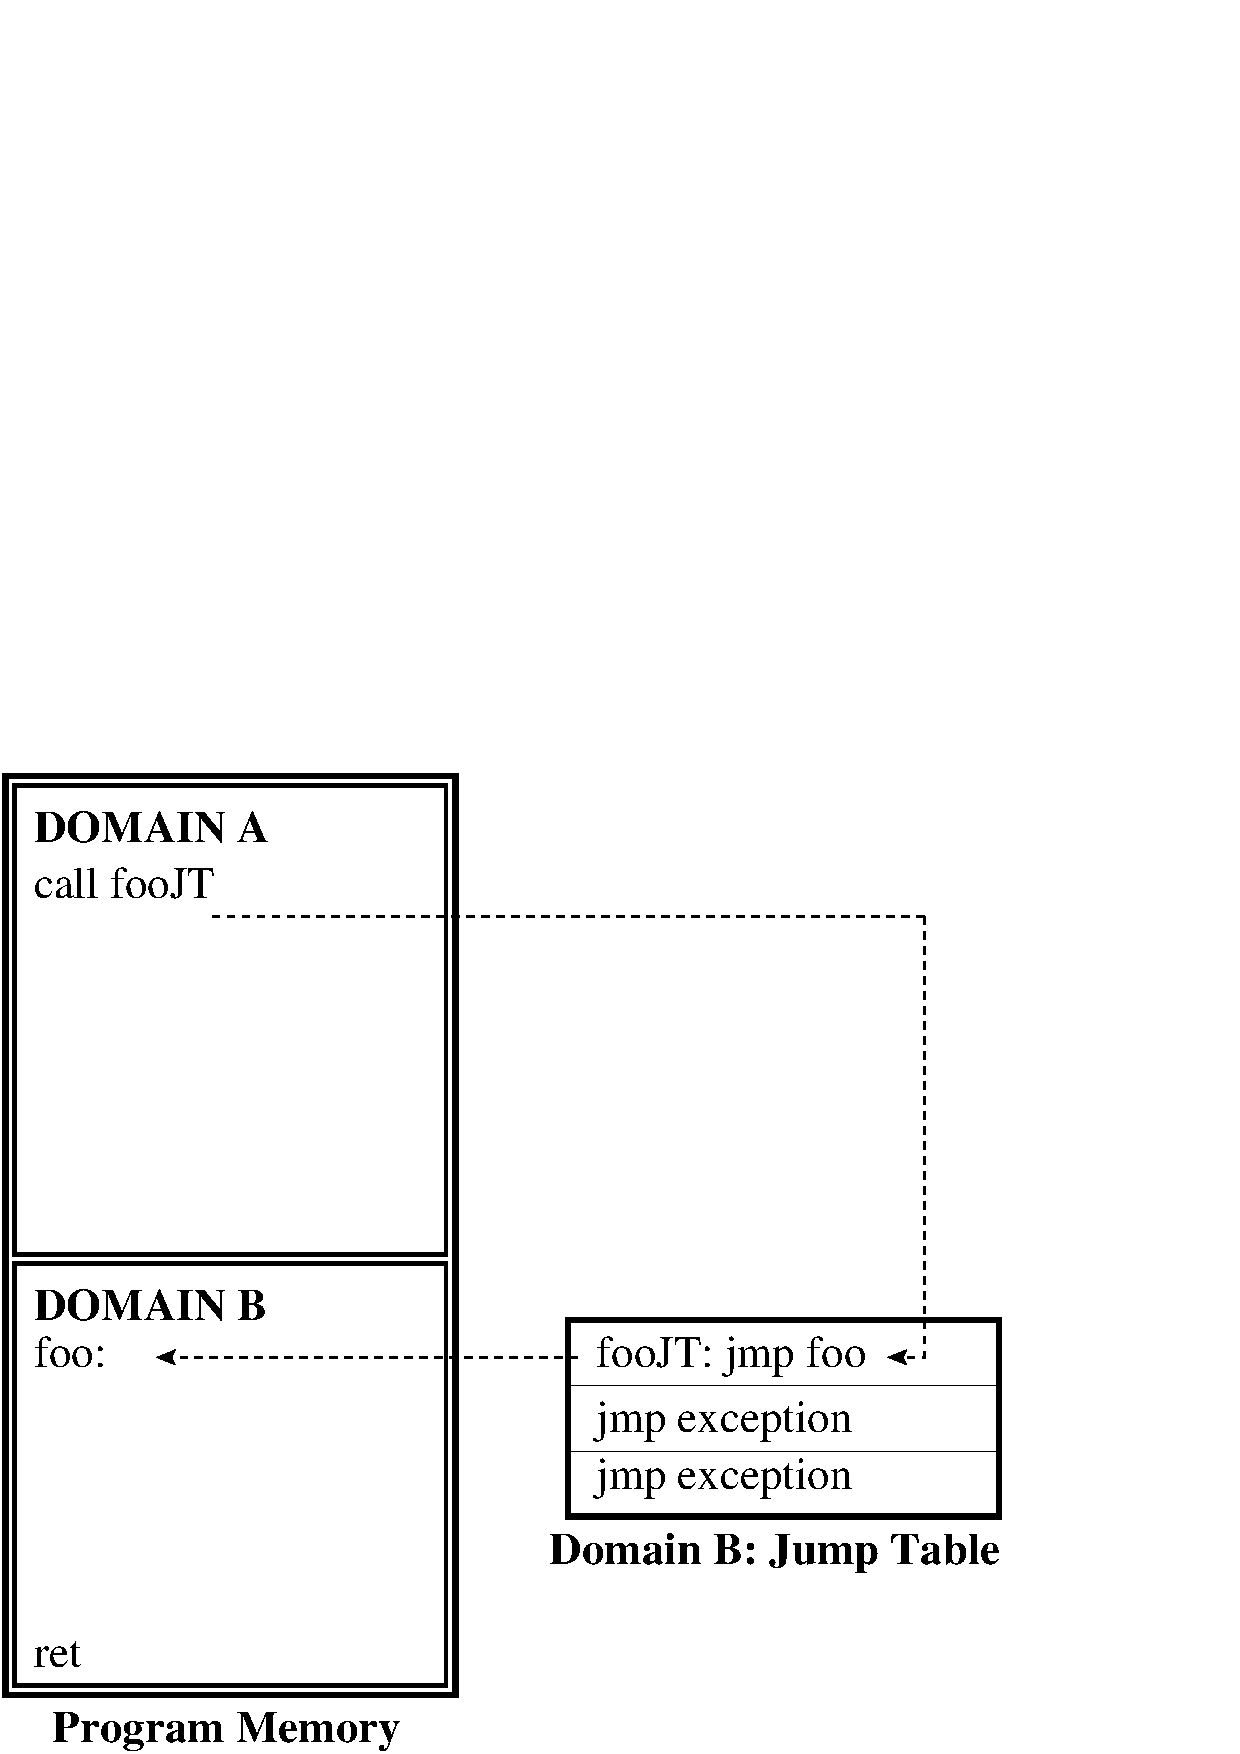
\includegraphics[height=1.75in, keepaspectratio=true]{figures/cross_domain_call.pdf} 
   \caption{Cross Domain Linking}
   \label{fig:cross_domain_call}
\end{figure}
%
%==============================================================================================
% DOMAIN TRACKING
%==============================================================================================
\subsection{Domain Tracking}
%
Domain tracking is performed in hardware by extending the implementation of \texttt{call} and \texttt{return} instructions.
%
Each domain is allocated one complete page of flash memory to store its jump table.
%
In the AVR architecture this imposes a limit of 128 functions that can be exported by every domain.
%
This limit can be easily extended by allocating more space to the jump table.
%
%The maximum number of exported functions by any SOS module is 12.
%
Empty entries in the jump table are filled with a jump instruction to an exception routine.
%
Jump table pages of all domains are co-located and stored at fixed location in flash memory.
%

This organization simplifies the algorithm for verifying the target address of a call.
%
A valid target address has to reside in the jump table.
%
This is checked by a simple compare operation to the base address of the jump table.
%
The check against the upper bound of jump table is deferred.
%
%and stack bound need to be stored in a stack.


The identity of the called domain is also easily determined.
%
Jump tables of all domains are organized linearly, starting from the domain 0 jump table located at the base address.
%
The identifier of the target domain can be easily determined by first computing the address offset from the base address of the jump table and dividing it by the size of the jump table.
%
If the target domain identifier exceeds the maximum number of domains in the system, then it indicates that the target address is greater than the upper bound of the jump table, and an exception is generated.
%
Finally, a call is made into the jump table that is redirected to the actual entry point in the target domain.
%

The current domain identifier needs to be pushed to a stack, because cross domain calls can be chained: domain A calls domain B which in turn calls domain C.
%
During cross domain return, the previous domain identifier is restored and the control is transferred back to the caller's domain.
%
The cross domain state machine handles the push and pop operations transparently to the application programs.
%
%All function calls made across domains pass through a \textit{jump table} setup in the program memory.
%
%Four operations are performed by the cross domain call stub.
%
%First, it verifies target address of the call.
%
%A valid target address should match the address of any exported function.
%
%Second, it determines the identity of callee domain and stores it.
%
%Third, it saves the return address of caller domain.
%
%Fourth, it sets up a stack bound.
%
%Stack bound is required for stack protection (Section~\ref{subsec:stackguard}).
%
%Cross domain call stub resides within the single trusted domain.
%
%Design of calling mechanism tries to optimize performance overhead of these operations.
%
%
%==============================================================================================
% STACK PROTECTION
%==============================================================================================
\subsection{Run-Time Stack Protection}
\label{subsec:stackguard}
%
Embedded micro-controllers have a single execution stack that is shared by the entire system.
%
In most architectures, the stack is initialized at the end of address space and grows down towards the start of address space.
%
The run-time stack is used for many purposes.
%
First, it is used to record the return addresses of function calls.
%
Second, it is used to set up data frames for storing local variables or function arguments that cannot be accommodated in registers.
%
Third, it is also used to store arguments for variadic functions.
%
Stack corruption is a serious problem.
%
Our protection model prevents corruption of the stack belonging to one domain by any module belonging to a different domain.
%
During a cross domain call  the processor copies the current stack pointer into a \texttt{stack\_bound} register. 
%
The previous stack bound is saved.
%a stack bound is setup before control is transferred from one domain to another.
%
The memory map checker compares the write address to the current stack bound and signals an exception if the address exceeds the stack bound.
%disallows writes to memory addresses greater than current stack bound.
%
%As shown in figure~\ref{fig:checker}, stack access checker is invoked if the write address points to stack.
%
%Stack access checker 
%
Therefore, modules belonging to a domain cannot corrupt the stack belonging to another domain.
%
%==============================================================================================
% SAFE STACK
%==============================================================================================
\subsection{Safe Stack}
%
A module can call any local function within its domain.
%
The return address of function calls are stored in stack and are protected from corruption from modules in other domains.
%
However, a programming error can cause a module to corrupt its own stack.
%
This cannot be prevented by protection domains.
%
Therefore, we store all return addresses in a separate stack that resides in a different protection domain.
%
We call this a safe stack.
%
%Entry (and exit point) of every local function in a domain is re-written to invoke a stub routine that pushes (and pops) return addresses into the Safe Stack.
%
%Safe Stack pointer is maintained as a global variable that is read (and written) before (and after) a sequence of push/pop operations. 
%
%Safe Stack is used to overwrite return address values in run-time stack.
%
%We do not modify run-time stack in any manner as it would corrupt data frames setup by functions for storing local data and function arguments.
%
A safe stack can be setup only by the software in the trusted domain by writing to the \texttt{safe\_stack\_ptr}.
%
The safe stack can be setup anywhere in data memory as long as it is protected from accidental writes and overflow.
%
We usually setup Safe Stack at the end of all global data in the system and make it grow upwards.
%
Run-Time stack and Safe Stack approach one another.
%
%Binary rewriter introduces the stubs to push and pop into Safe Stack.
%
%Therefore, all return addresses are checked.
%
%Domains occupy contiguous portions in program memory. 
%
%When the domain is loaded into a system, the Control flow manager records its start and end addresses.
%
%Return addresses are checked to ensure that they lie within bounds of the current domain; else an exception is raised.
%
%Similarly, all computed call addresses are also subject to an identical bounds check.
%
%Calls to static addresses are verified at load time.
%
%All checks are introduced through a binary rewriter.














%=========================================================================
% EVALUATION
%=========================================================================
\section{Evaluation}
\label{sec:eval}
In this section, we will analyze the protection benefits and overheads introduced by our methodology.
%
We have implemented the hardware components of our design by making extensions to the AVR instruction set architecture.
%
The VHDL model of the extended processor is synthesizable.
%
We have instantiated the processor on Xilinx Vertex 2 Pro XC2VP30 FPGA.
%
Our performance overheads are measured using Modelsim 6.0 simulator.
%
The software library and applications were compiled using \texttt{avr-gcc} cross compiler.
%
%\subsection{Micro-Benchmarks}
%
\subsection{Performance Overhead}
%
We first present micro-benchmarks that measure CPU overhead introduced by the protection mechanism.
%
Table~\ref{tab:microbmperf} contains the overhead of run-time checks present in our mechanism.
%
We compare our overhead with a completely software based approach to memory protection through binary rewrites proposed in~\cite{ram07harbor} for the AVR architecture.
%
The software based approach also introduces identical run-time checks except that they are implemented in assembly language without any modifications to the processor architecture.
%
The results clearly indicate the superior performance of run-time checkers implemented in hardware.
%
\begin{table}[htdp]
\centering
\small{
\begin{tabular}{|l|c|c|}
	\hline
	Function Name & AVR Extension & AVR Binary Rewrite\\
	\hline
	Memmap Checker & 1 & 65\\
	Cross Domain Call & 5 & 65\\
	Cross Domain Ret & 5 & 28\\
	Save Ret Addr & 0 & 38\\
	Restore Ret Addr & 0 & 38\\
	\hline
\end{tabular}}
\caption{Overhead (CPU cycles) of Memory Protection Routines}
\label{tab:microbmperf}
\end{table}
%

The high overhead of software based memory map checker is mainly due to complex bit shift operations that are required to translate write addresses to memory map lookup.
%
Cross domain call and return have an overhead of five clock cycles when implemented in hardware.
%
The overhead occurs because the current domain identity, stack bound and return address have to be pushed to the safe stack before they can be updated with new values.
%
The total information that needs to be pushed to the stack is five bytes and only one byte can be written every clock cycle.
%
Similarly on the cross domain return, the five clock cycles are expended in restoring the values read from the safe stack.
%
Saving and restoring return addresses to the safe stack does not introduce any added overhead.
%
This is because the hardware unit for safe stack simply takes over the address bus when the processor is pushing the return address to the run-time stack.
%
By stealing the address bus from the processor, the hardware unit is able to simply redirect the store of the return addresses to the safe stack.

Next we evaluate the software library.
%
Performance overhead is also introduced by updates to memory map during allocation, free and transfer of memory within the system.
%
Table~\ref{tab:malloc_comparison} compares the overhead of memory allocation routines in the presence and absence of the protection mechanism.
%
Relatively higher overhead of \texttt{change\_own} and \texttt{free} calls is due additional checks that are introduced to prevent illegal ownership transfer or freeing of memory blocks by non-owners.
%
\begin{table}[htdp]
\centering
\small{
\begin{tabular}{|l|c|c|}
	\hline
	Function Name & Normal & Protected \\
	\hline
	malloc  & 343 & 610\\
	free & 138 & 425\\
	change\_own & 55 & 365 \\
	\hline
\end{tabular}}
\caption{Overhead (CPU cycles) of memory allocation routines}
\label{tab:malloc_comparison}
\end{table}
%

\subsection{Resource Utilization}
%
Resource utilization can be partitioned into sections.
%
The resource utilization of the software library and the overhead of hardware checkers.
%

%
%Code memory usage increases by about 15\% in protected kernel relative to unprotected kernel.
%
%Increase is mainly due to memory map API and jump table used by cross domain call mechanism.
%
%There is no significant change in program memory usage going from two protection domains to multiple protection domains.
%
%Data memory usage increases by 5\% and 9.5\% in two-domain and multi-domain systems respectively, relative to unprotected kernel.
%
%This is the maximum possible overhead as the memory map stores layout and ownership information of entire address space.
%
Code and data memory usage of the software library is shown in Table~\ref{tab:swlibsize}.
%
Maximum memory map size is 256 bytes for multi-domain protection.
%
This represents an overhead of 6.25\%.
%
However, by modifying data layout, portion of address space that requires memory map for protection can be reduced.
%
For example, memory map can be configured only to protect the heap and safe-stack.
%
By abutting these two data-structures, size of memory map required can be reduced to 140 bytes for multi-domain protection.
%
For two domain protection, the overhead can be reduced to only 70 bytes (1.7\%).
%
The total code memory usage of the software library is only 3674 bytes (2.8\%).
%
\begin{table}[htdp]
\centering
\small{
\begin{tabular}{|l|c|c|}
	\hline
	SW Component & FLASH (B) & RAM (B)\\
	\hline
	Dynamic Memory & 1204 & 2054\\
	Memory Map & 422 & 256 \\
	Jump Table & 2048 & 0 \\
	\hline
\end{tabular}}
\caption{FLASH and RAM overhead of software library}
\label{tab:swlibsize}
\end{table}
%

The hardware overhead of our mechanism is shown in Table~\ref{tab:hwsize}.
%
These results were computed by synthesizing our processor on Xilinx ISE 8.2i.
%
Most of the additions to the core area are in the memory map decoder that maintains a barrel shifter to support arbitrary bit-shifts in a single clock cycles.
%
We can eliminate this overhead if the processor is synthesized for a fixed block size and number of protection domains.
%
The overall increase in the core area is about 32\%.
%
This represents a modest increase in the overall area of the chip as the core occupies only a small fraction of the overall area.
%
Bulk of the chip area is occupied by SRAM and FLASH memories.
%
\begin{table}[htdp]
\centering
\small{
\begin{tabular}{|l|c|c|}
	\hline
	HW Component & Ext. Gate Count & Orig. Gate Count\\
	\hline
	AVR Core & 22498 & 16419\\
	Fetch Decoder & 6783 & 6685\\
	MMC & 2284 & N/A \\
	Safe Stack & 1749 & N/A \\
	Domain Tracker & 541 & N/A \\
	\hline
\end{tabular}}
\caption{Gate count overhead of hardware extensions}
\label{tab:hwsize}
\end{table}
%







%%%%%%%%%%%%%%%%%%%
% Related Work
%%%%%%%%%%%%%%%%%%%
\section{Related Work and Background}
\label{sec:related}
%
This section reviews other systems that provide memory protection.
%
The systems are broadly classified based on their application
domains.
%
We focus first on sensor networks and then survey the more general
space of desktop and server computing systems.
%
%We conclude this section with a brief overview of SOS operating system.
%
%=====================================================================
\subsection{Sensor Networks}
%
As sensor networks are envisioned for long-term deployments, several
projects have addressed reliability as a primary design
concern~\cite{tkernel06sensys,regehr06utos,dutta05ipsn}.
%-------------------------------------------------------------
\subsubsection{Naturalization --- \emph{t-kernel}}
%
\emph{t-kernel}~\cite{tkernel06sensys}, a runtime for Mica motes, also
rewrites binaries to make them safe for execution.
%
Harbor and \emph{t-kernel} represent different points in the design space of
software-based protection mechanisms.
%
\emph{t-kernel} enforces a strong isolation boundary between the application and
the kernel.
%
Through a process called \emph{naturalization}, the application binary is
rewritten on the sensor node to guarantee that the \emph{t-kernel} can
always safely regain control of the processor, even, for example, in the
presence of application infinite loops that could otherwise hang the
system.
%
The rewritten application binary contains an entire TinyOS operating system
image, in contrast to Harbor, where multiple modules within an
application are prevented from corrupting one another.
%


\emph{t-kernel} also implements software-based differentiated
virtual memory,
%
which translates the addresses for all memory accesses made by a program
into the heap segment.
%
The overhead of virtual memory is unpredictable and can be very
high in the event of a swap from external flash.
%
Harbor does not implement virtual memory, but does enforce memory isolation at a
finer granularity than \emph{t-kernel}.
%
In particular, Harbor can protect application modules from
one another.
%

Harbor does not address control flow isolation, except as required to
enforce memory isolation; in particular, it cannot force a buggy module
stuck in an infinite loop to relinquish control of the CPU.
%
\emph{t-kernel} requires external flash memory, whereas Harbor makes use of
on-chip flash memory only.
%
%-------------------------------------------------------------
\subsubsection{Safe OS Extensions --- UTOS}
%
Safe TinyOS~\cite{regehr06utos} uses CCured~\cite{ccured02necula} and static
analysis techniques to provide memory safety for TinyOS applications.
%
CCured performs complex pointer analysis to mark pointers as safe or
unsafe.
%
Much driver code performs arbitrary typecasts that can cause CCured to
fail or conservatively mark pointers as unsafe, which introduces a
performance penalty as the CCured run-time performs bounds checks on
unsafe pointers during code execution.
%
CCured provides memory safety at a much finer granularity than Harbor.
%

The UTOS framework allows untrusted extensions to
safely interface with Safe TinyOS components.
%
UTOS extensions are made type-safe and memory-safe using CCured and a
backend service that copies buffers when they are exchanged between the
extension and the Safe TinyOS core.
%
Extensions are not allowed to interact with one another.
%
Harbor allows safe buffer transfers without copying, and allows extensions
to interact, but its current simple runtime check infrastructure introduces
overhead that CCured can sometimes avoid.
%

The UTOS backend service also mediates resource requests and prevents any
extension from starving other extensions in the system.
%
Harbor does not make any guarantees on fair resource allocation.
%
%-----------------------------------------------------------------
\subsubsection{Application Specific Virtual Machines --- Mat\'e}
%
Application Specific Virtual Machines (ASVM) such as
Mat\'e~\cite{asvm05nsdi}~\cite{levis02mate} and
Agilla~\cite{agilla05ipsn} are domain specific interpreters that
execute high-level application scripts.
%
Both Harbor and ASVMs provide memory safety to applications, albeit
through different mechanisms.
%
Harbor isolates applications from one another.
%
ASVM performs type and bounds checks on all memory accesses.
%
ASVM's checks are in some ways more stringent than Harbor's protection,
since the type safety of the instruction set also prevent scripts from
corrupting \emph{their own} memory.
%
However, errors in ASVM's native code implementation might corrupt any
memory on the node.
%
Further, for efficiency, ASVMs are designed to be easily extensible to
customize the interpreters for a specific application domain.
%
The extensions can also be introduced dynamically~\cite{balani06dvm}.
%
The ASVM extensions implement powerful high level opcodes that perform
complex operations.
%
The extensions are implemented in non-type safe languages and can be
buggy.
%
ASVMs could thus use Harbor's isolation to become more robust to errors in
extensions.


The trade-offs between ASVMs and Harbor are evaluated in detail in
Section~\ref{sec:eval}.
%
Harbor has a significantly lower execution overhead compared than ASVM,
%
but its run-time checks 
%introduced by Harbor 
increase code size.
%
%-----------------------------------------------------------------
\subsubsection{Type Safe Languages --- Virgil}
%
Type-safe languages provide memory safety at a fine granularity.
%
Type-safe languages for resource constrained microcontrollers is an
emerging area of research.
%
Most of the software developed for embedded systems is written in
unsafe languages such as C (or even assembly for low-level drivers). 
%
%The popular sensor network programming language NesC~\cite{gay03nesc}
%contains minimal extensions to C (such as the \texttt{atomic} keyword)
%to prevent race conditions.
%
%However, it does not address memory safety.


A common criticism of safe languages or unsafe languages retrofitted
with type information~\cite{ccured02necula} is their excessive CPU and
memory consumption.
%
This often makes them unsuitable for resource constrained sensor
nodes.
%
Virgil~\cite{titzer06virgil} is a new programming language that
attempts to address some of these concerns.
%
By explicitly separating initialization time from run time, Virgil
allows an application to build complex data structures during
compilation and then run directly on bare hardware without a virtual
machine or a language run time.
%
The separation allows the entire program heap to be available at
compile time and enables new optimizations that reduce memory size.
%
Virgil does not support dynamic memory allocation.
%
Therefore, it is currently suited for building application specific
static operating system images such as TinyOS~\cite{levis05t2}.
%
An interesting area of future research is to explore safe languages
(such as Virgil) as a primary extensibility mechanism for dynamic
sensor operating systems such as SOS~\cite{ram05sos}.
%
%SPIN project~\cite{spin95sosp} at University of Washington explored
%safe languages as the primiary extensibility mechanism in desktop
%operating systems.

Finally, a safe language restricts an implementation to a single
language; it ignores a large base of existing code.
%
Harbor operates on compiled binaries and is therefore independent of
any programming language and is applicable to all existing code.
%
Type safe languages require unsafe extensions to interface to
low-level hardware\footnote{Virgil extends type safety to the
  hardware}, though these extensions could be used sparingly.
%
Another problem with type-safe languages is the size of the system
that needs to be trusted.
%
A complete language compiler and run-time consists of an optimizer
that uses complex analysis to improve run-time efficiency.
%
This is a large and complicated code base, all of which needs to be
trusted.
%
In contrast, for Harbor, only the run-time components and the simple
verifier needs to be trusted.
%
The size of this system is considerably smaller than the size of a
compiler.
%
% VM*~\cite{vmstar05sensys} is a virtual machine construction kit
% targets resource constrained sensor nodes and supports a subset of the
% JAVA programming language.
% %
% The VM* framework automatically generates an application specific
% virtual machine.
% %
% The virtual machine is optimized to include only parts of the
% interpreter and the run-time that are needed.
% %
% A native API exposes the OS and hardware services to the JAVA
% applications.
% %
% VM* addresses the development of applications in JAVA but the
% underlying operating system and device drivers are still written in
% non type-safe languages such as C or assembly.
% %
% JAVA applications in VM* are type-safe.
% %
% Unlike Harbor and UTOS, the VM* applications are not isolated from the
% operating system.
%
%Sympathy, a debugging framework, has focussed on developing
%network-level protocols to diagnose/localize
%problems~\cite{nithya05sympathy} 
%
%We can leverage Sympathy framework to send diagnostic information to
%the basestation whenever an exception is triggered in Harbor
%
%At present, hardware support in sensor nodes to achieve high
%dependability is absent, with reboot of the entire node being the
%most common approach~\cite{dutta05ipsn}.
%
%

Recently, RETOS operating system~\cite{retos07spots}, also provides
memory protection for applications through a rewrite of compiled binary.

%=========================================================================
\subsection{Software-based Techniques}
%
The design considerations for an embedded sensor system are vastly
different from a desktop/server system.
%
Still, some of the features in Harbor have been motivated from the
large range of software-based memory protection techniques proposed
for desktop/server systems.
%
%------------------------------------------------------------
\subsubsection{Software-based Fault Isolation (SFI)}
\label{subsec:sfi}
%
Software-based Fault Isolation (SFI) is a general technique that
restricts the address range of stores, jumps and calls by modifying a
program binary.
%
The key challenge to SFI is to introduce the restrictions efficiently, and in
a manner that they cannot be bypassed by maliciously designed input
code.
%
SFI was originally proposed by Wahbe et al.~\cite{wahbe93sfi} (called
``sandboxing'').
%
%The pseudocode to sandbox an address is explained in
%Figure~\ref{fig:sbxpseudocode}.
%
%
% \begin{figure}
%  \begin{tabbing}
%   \texttt{dedi}\=\texttt{cated-reg} $\Leftarrow$ \texttt{target-reg \&
%     and-mask-reg} \\
%   \>\emph{Use dedicated register} \texttt{and-mask-reg} \emph{to clear
%     segment identifier bits.}\\
%   \texttt{dedicated-reg} $\Leftarrow$ \texttt{target-reg |
%     segment-reg} \\
%   \>\emph{Use dedicated register} \texttt{segment-reg} \emph{to set
%     segment identifier bits.}\\
%   \texttt{store instruction uses dedicated-reg}
%  \end{tabbing}
%  \caption{Assembly pseudo code to sandbox address in
%    \texttt{target-addr}}
%  \label{fig:sbxpseudocode}
% \end{figure}
% %

Sandboxing enforces static partitioning on an application's virtual address
space to enable safe sharing of the address space by multiple
cooperative modules.
%
By choosing address space boundaries to be powers of 2, sandboxing
restrictions are efficiently introduced through bit-masks.
%
%Specifically, the target address of a store instruction is forced to belong to its domain.
%
Dedicated registers guarantee that checks cannot be bypassed by
jumping into the middle of a sandbox sequence.
%
In addition, Wahbe et al. also designed a low-latency
cross-fault-domain communication mechanism.
%

Harbor strives to enforce similar restrictions as SFI; it disallows
stores and jumps to addresses outside the module's domain.
%
However, the architectural limitations of the embedded processors
motivate new design approaches.
%
First, the absence of virtual memory in embedded processors limits the
total address space to the available physical memory.
%
The on-chip SRAM in AVR microcontroller~\cite{avrdatasheet} is a meagre 4 Kb.
%
Therefore, static partitioning of the physical memory address space is
infeasible; it would lead to excessive internal fragmentation of the
limited memory.
%
Second, all software domains on an embedded processor share a
common run-time stack.
%
SFI implementations for desktop processors set up a separate stack for
each domain within their allocated address space.
%
Protecting the shared run-time stack is a design challenge for Harbor.
%
Third, the instruction set architectures of embedded processors have
limited capabilities.
%
For instance, in AVR, the load and store operations can use only three
pairs of registers for addressing.
%
Therefore, it is often infeasible to set aside a dedicated register
pair for sandboxing.
%
Techniques different from SFI have to be employed to ensure that
Harbor checks are not circumvented.
%
Fourth, there is no support for privileged instructions in an embedded
processor.
%
Since embedded software runs directly ``on metal'', therefore Harbor
has to detect and disallow certain potentially unsafe opcodes, such
as store to program memory.
%


Many variations of SFI have emerged since Wahbe's original
implementation of this technique for the two RISC architectures, MIPS
and Alpha.
%
In particular, the x86 implementations of SFI also face one similar
constraint as Harbor, namely the lack of sufficient registers in the
architecture to set aside a dedicated register.
%
MiSFIT~\cite{small97misfit}, an assembly language re-writer designed
to isolated faults in C++ code written for an extensible operating
system, uses a hash table of legal jump targets.
%
Control flow is re-directed through a check that ensures that jump
targets appear in the hash table.
%
This eliminates the need for dedicated registers.
%
PittSFIeld~\cite{pittsfield} divides the program memory into chunks of
16 bytes\footnote{Any size that is a power of 2 would suffice.} and
ensures through padding with \texttt{NOPS} that control flow does not
change except at an entry or exit of a chunk boundary.
%
The sandboxing sequence is inserted entirely within a chunk and
therefore cannot be circumvented.


\subsubsection{Control Flow Integrity (CFI)}
%
A Control Flow Integrity (CFI)~\cite{cfi05msr} policy dictates that
software execution must follow the path of a \emph{control flow graph}
(CFG) determined ahead of time.
%
CFI has more general goals than SFI, which focuses solely on restricting a
program's jumps.
%
CFI is implemented by labelling each potential jump target by a
uniquely encoded tag symbol.\footnote{Tag symbol is decoded as
  \texttt{NOP}.}
%
All computed control transfers check for the appropriate tag before
transferring control.
%
XFI~\cite{xfi06osdi} builds on CFI to offer a
flexible, generalized and more efficient form of SFI.
%
Further, XFI uses a two-stack execution model to ensure verifiable
control flow integrity.
%The two-stack execution model used by Harbor to ensure module control flow
%integrity was motivated by XFI~\cite{xfi06osdi}, a high-performance variant
%of SFI.
%
XFI's scoped stack holds data accessible only in the static scope of
each function, including return addresses and most local variables.
%
A separate allocation stack stores data that may be shared within the
functions in a module.
%
The two-stack execution model used by Harbor for ensuring control flow
integrity within a module was motivated by XFI.
%
%--------------------------------------------------------------------
\subsubsection{Safe OS Extensions}
%
Our work is also related to several other efforts in the
desktop/server space to isolate kernel modules such as device drivers,
either using hardware support (Nooks)~\cite{swift05nooks} or through type-safe
languages (SPIN)~\cite{spin95sosp} or software fault isolation
(exokernel)~\cite{exo97sosp}.
%
Nooks separates modules into lightweight protection domains by
managing separate page tables for each module.
%
Our approach is similar to Nooks in that it maintains memory ownership
information.
% and relies on standard interfaces to control flow and access of
% resources.
%
%=======================================================================
\subsection{Hardware-based Approaches}
%
We review the current state of the art in hardware based memory protection
and compare it with UMPU, our hardware-assisted fault isolation system.
%
\subsubsection{Memory Management Unit (MMU)}
%
Page-based virtual memory systems have become the dominant form of
memory management in the modern general-purpose computer systems.
%
The coarse granularity of page-based protection, its high performance
overhead, and its complexity does not make it popular in low-end
embedded microcontrollers.
%
%
\subsubsection{Memory Protection Units (MPU)}
\label{sec:mpu}
%
A Memory Protection Unit (MPU) is used to statically partition memory
and set individual protection attributes for each partition.
%
The partitions are contiguous segments within the address space
defined by a pair of base and bounds registers.
%
The most common protection attributes are shown in
Table~\ref{tab:armprotattr}.
%
\begin{table}[htdp]
\centering
\small{
\begin{tabular}{|c|l|}
	\hline
	Code & Mode Description\\
	\hline
        00 & No Access \\
        01 & Privileged Mode Access Only \\
        10 & Privileged Mode Full Access, User Mode Read Only \\
        11 & Full Access\\
	\hline
\end{tabular}}
\caption{ARM940T Protection Attributes Descriptions}
\label{tab:armprotattr}
\end{table}
%

The MPU protection model is not suited for embedded sensor
software running on low-end microcontrollers.
%
MPU defines only two protection domains, user mode and supervisor
mode.
%
This is sufficient for protecting the kernel from applications, but
not applications from one another.
%
The static partitioning of the address space into contiguous regions is
infeasible for the low-end microcontrollers with very limited memory
footprint.
%
Further, the number of partitions is also limited.
%

However, MPU has a lower memory footprint than UMPU because the
partitioning information can be stored in registers instead of
maintaining a memory map.
%
MPU introduces no performance overhead while UMPU incurs a single
clock cycle penalty for memory map accesses.
%
MPU's are used in embedded processors such as ARM
940T~\cite{arm940tds} and Infineon TC1775~\cite{inftc1775ds}.
%--------------------------------------------------------------------
\subsubsection{Mondriaan Memory Protection}
%
Mondriaan Memory Protection (MMP)~\cite{witchel-asplos02-mondrian}
creates hardware enforced protection domains within a single address
space.
%
MMP inspects memory accesses at the instruction level from within the
processor pipeline to provide word-level protection.
%
MMP is designed for high performance desktop architectures and it uses
fairly complex and expensive hardware extensions to reduce overhead of
monitoring all accesses.
%
MMP also maintains a table of access permissions within memory for
every address space.
%
However, the tables are significantly larger that Harbor memory map as
MMP protection is more flexible and fine-grained.
%
Further, as chip area and cost are not dominant concerns, MMP
implements an expensive Protection Lookaside Buffer (PLB) to reduce
the overhead of checks introduced during memory accesses.
%
%------------------------------------------------------------------
\subsubsection{Hardware Accelerated Checkers}
%
Divya et al.~\cite{divya06ccured} propose a system that enhances the
CCured~\cite{ccured02necula} run-time checks by performing them in
hardware.
%
A group of \texttt{XCHECK} custom instructions are added to the
Xtensa~\cite{xtensads}, a customizable processor from Tensilica Inc.
%
The \texttt{XCHECK} instructions are inserted into the CCured modified
source code using a source transformation tool.
%
UMPU has a similar motivation; using hardware accelerators for
improving performance.
%
UMPU does not enforce type safety, but focuses on fault isolation.
%
Therefore, the hardware accelerated CCured and UMPU enforce different
properties that can improve the reliability of embedded software.

%%%%%%%%%%%%%%%%%%%%%%%%%%%%%%%%%%%%%%%% 
% SOS Background
%%%%%%%%%%%%%%%%%%%%%%%%%%%%%%%%%%%%%%%% 
%\section{Background --- SOS Operating System}
% \subsection{SOS Operating System}
% \label{sec:background}
% % 
% The initial motivation of our work was to provide memory protection
% for mote-class sensor nodes running the SOS operating system.
% % 
% % The design ideas of Harbor are generally applicable however its
% % implementation and evaluation are specific to SOS.
% % 
% We have implemented and evaluated Harbor's protection mechanisms on
% SOS, although the ideas should apply elsewhere.
% % 
% This brief introduction to SOS is useful to fully understand the
% implementation of our scheme.
% % 
% %===================================================
% %\subsection{SOS Operating System}
% % 
% %% Unique resource tradeoffs in the nodes, the distributed and
% %% collaborative nature of applications and the remote unattended
% %% operation of sensor networks motivate the design of a new class of
% %% operating system and run-times.
% % 
% TinyOS~\cite{levis05t2}, the most popular operating system for sensor
% networks, uses reusable software components to implement common
% services, but each node runs a statically linked system image.
% % 
% %% The components are written in the NesC~\cite{gay03nesc} programming
% %% language.
% % 
% %% Mat\'e~\cite{asvm05nsdi}, an application specific virtual machine
% %% on top of TinyOS provides limited flexibility to re-task a deployed
% %% network using high-level scripts.
% % 
% SOS has a more traditional architecture: a kernel is
% installed on all nodes, and
% % 
% % The rest of the system and 
% application level functionality is implemented by a set of dynamically
% loadable binary modules~\cite{ram05sos}.
% % 
% % In contrast to TinyOS, SOS maintains modularity at the binary level
% % without any loss in efficiency.
% % 
% % This property of SOS makes it particularly attractive to explore
% % techniques for isolating software faults.
% % 
% %% We have implemented the memory protection mechanism on the SOS
% %% operating system.
% % 
% %% The embodiment of the scheme is specific to SOS, however it can
% %% easily be applied to the other existing run-times as well
% %% (subsection~\ref{sec:conclude}).
% % 
% % any operating system that supports dynamically loadable binary
% % modules.
% % 
% % This brief introduction to SOS is useful to fully understand the
% % implementation of our scheme.
% % 
% % 
% % 
% The kernel is relatively well tested; we assume it is free of
% programming errors.
% % 
% Modules are position independent binaries that implement a specific
% task or function, and are less well tested by comparison.
% % 
% Modules operate on their own state, which is dynamically allocated at
% run-time.
% % 
% An application in SOS is composed of one or more modules interacting
% via asynchronous messages or function calls.
% % 
% Examples of modules are routing protocols, sensor drivers, application
% programs, and so forth.
%
%----------------------------------------------------------
% \subsubsection{Module Linking}
% \label{sec:soslinking}
% %
% Any SOS module is linked upon loading with the kernel and other
% modules in the system. 
% %
% %Modules communicate with one another through asynchronous message
% %passing or synchronous function calls
% %(Figure~\ref{fig:sos_mod_interactions}).
% %
% The SOS kernel provides a rich set of services such as software
% timers, networking, sensor I/O, etc., accessible via a system
% call API.
% %
% The kernel maintains a jump table in program memory that stores the
% addresses of system calls (Figure~\ref{fig:sosjmptbl}).
% %
% The modules are pre-linked to the jump table entries.
% %
% Thus they do not have to carry any linking information, which reduces
% their size.
% %
% This design also provides flexibility to change the kernel independent
% of the modules as long as the consistency of the jump table is maintained.
% %

% Modules are also linked with one another through function pointer
% pointers (Figure~\ref{fig:modinteract}).
% %
% Every module carries records that indicates the set of functions to
% which it wishes to subscribe (from the rest of the system) and the set
% of functions that it provides (for the rest of the system).
% %
% The dynamic linker tracks down and links all the provide-subscribe
% function pairs when a module is loaded.
% %
% \begin{figure}[htpb]
%  \centering
%   \mbox{
%     \subfigure[Jump Table for System
%     API]{\label{fig:sosjmptbl}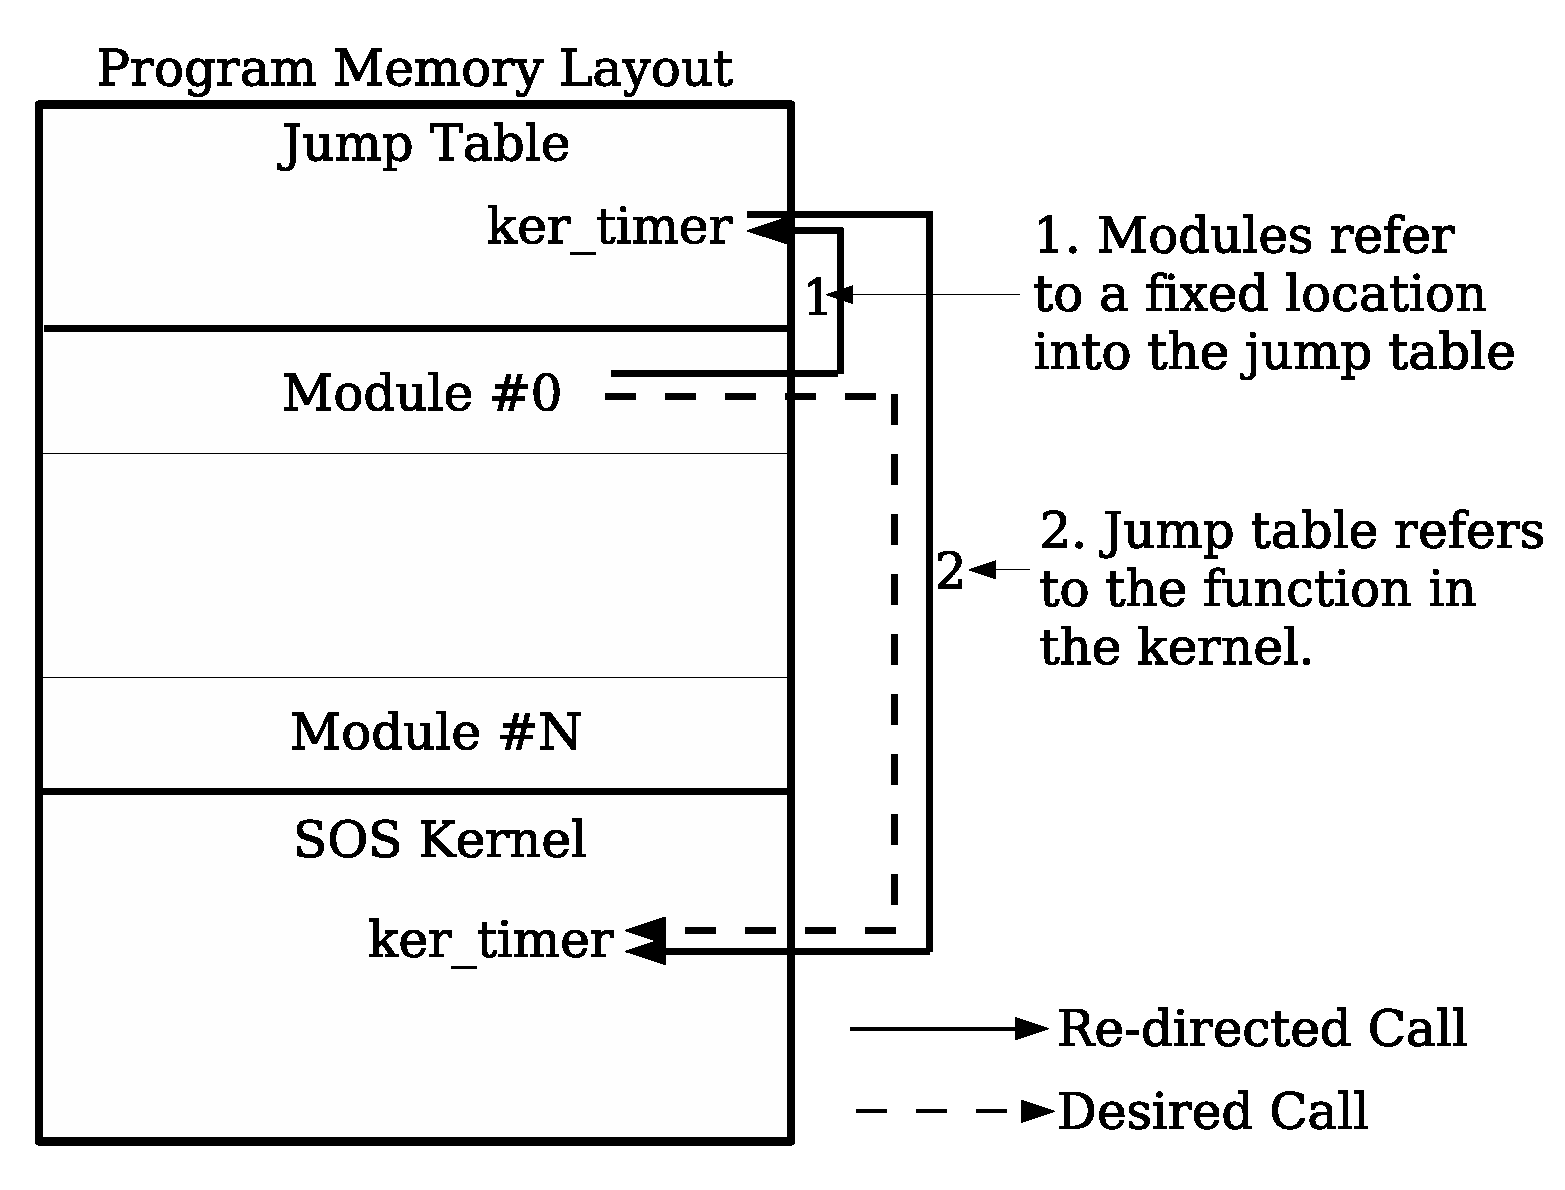
\includegraphics[width=2in,
%       keepaspectratio = true]{figures/jumptable.eps}}
%     \hspace{0.2in}
%     \subfigure[Module
%     Interactions]{\label{fig:modinteract}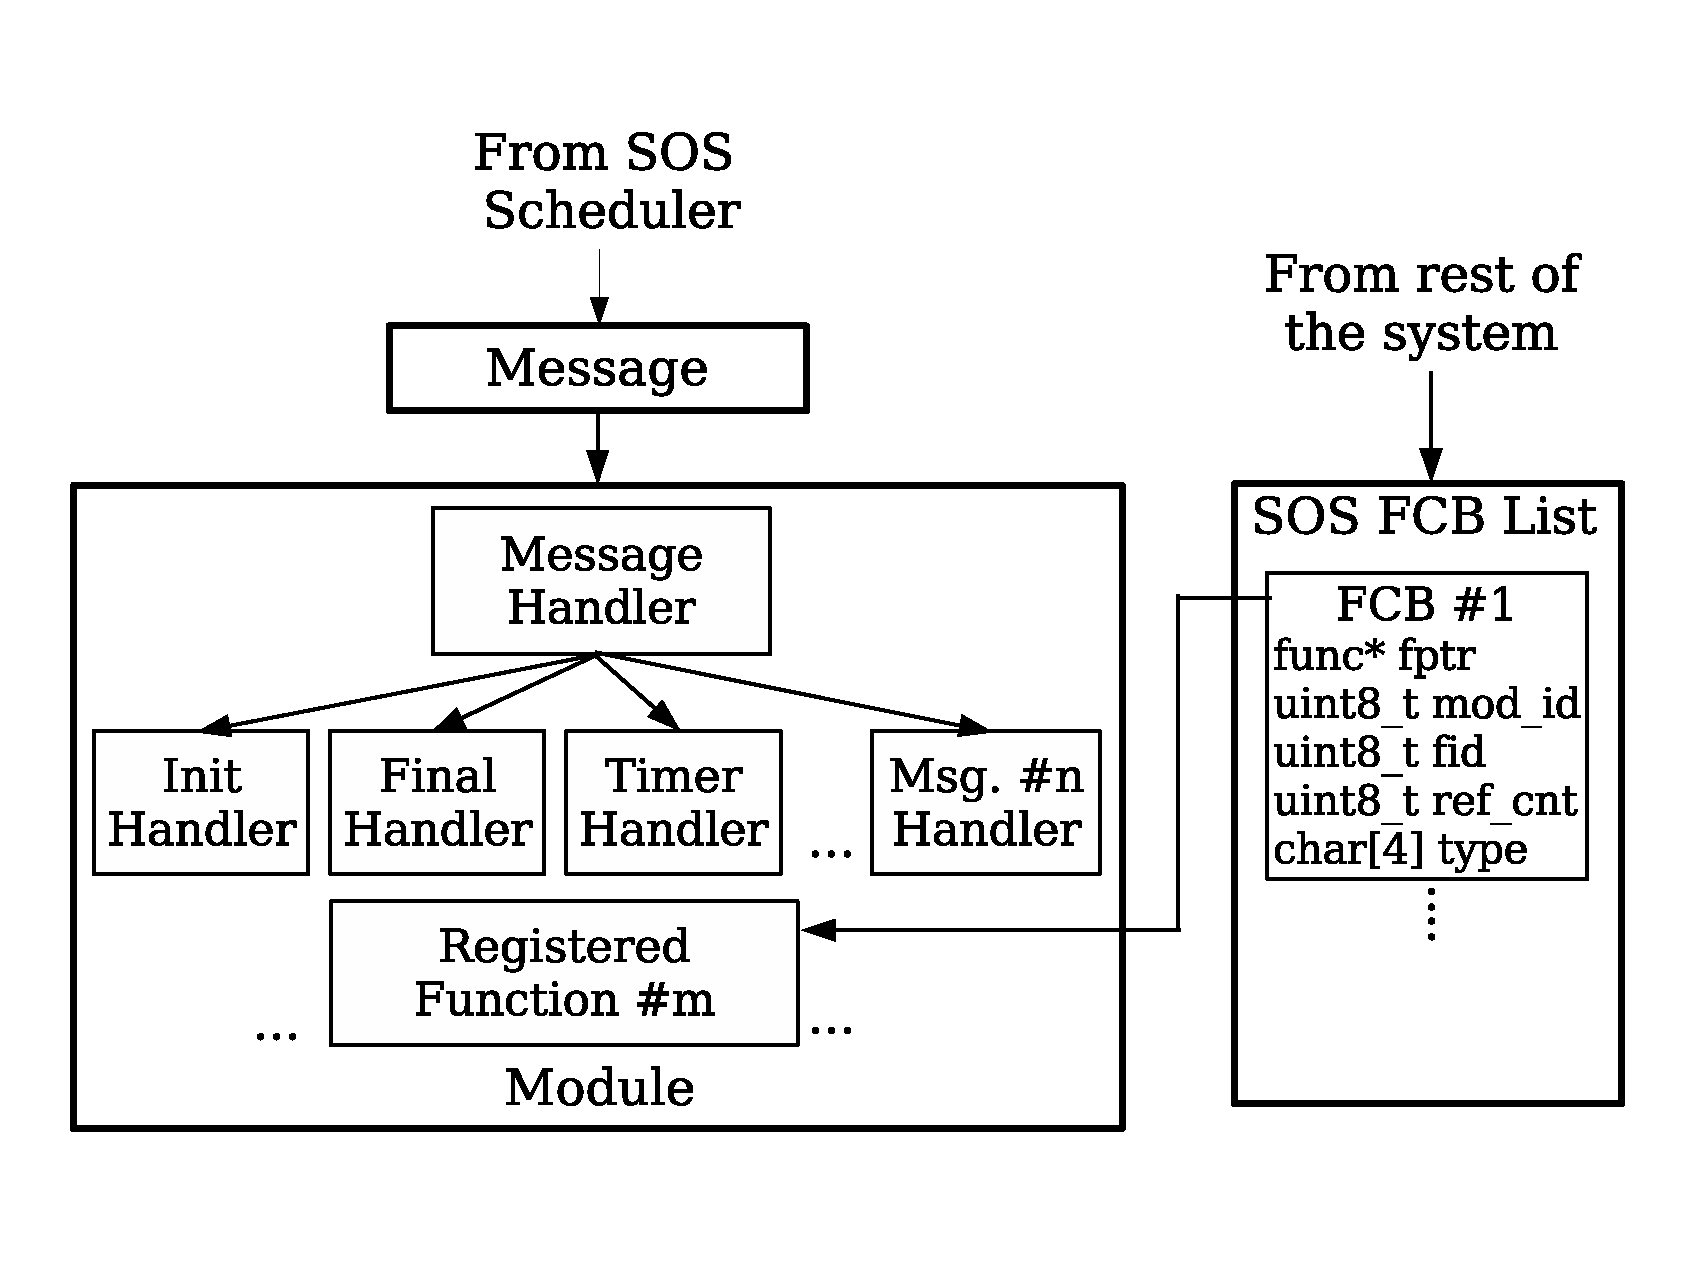
\includegraphics[width=2in,
%       keepaspectratio = true]{Figures/module_interactions.eps}}
%   }
%   \caption{Linking SOS Module}
% \end{figure}   
% %
% % \begin{figure}[htbp]
% %   \centering
% %   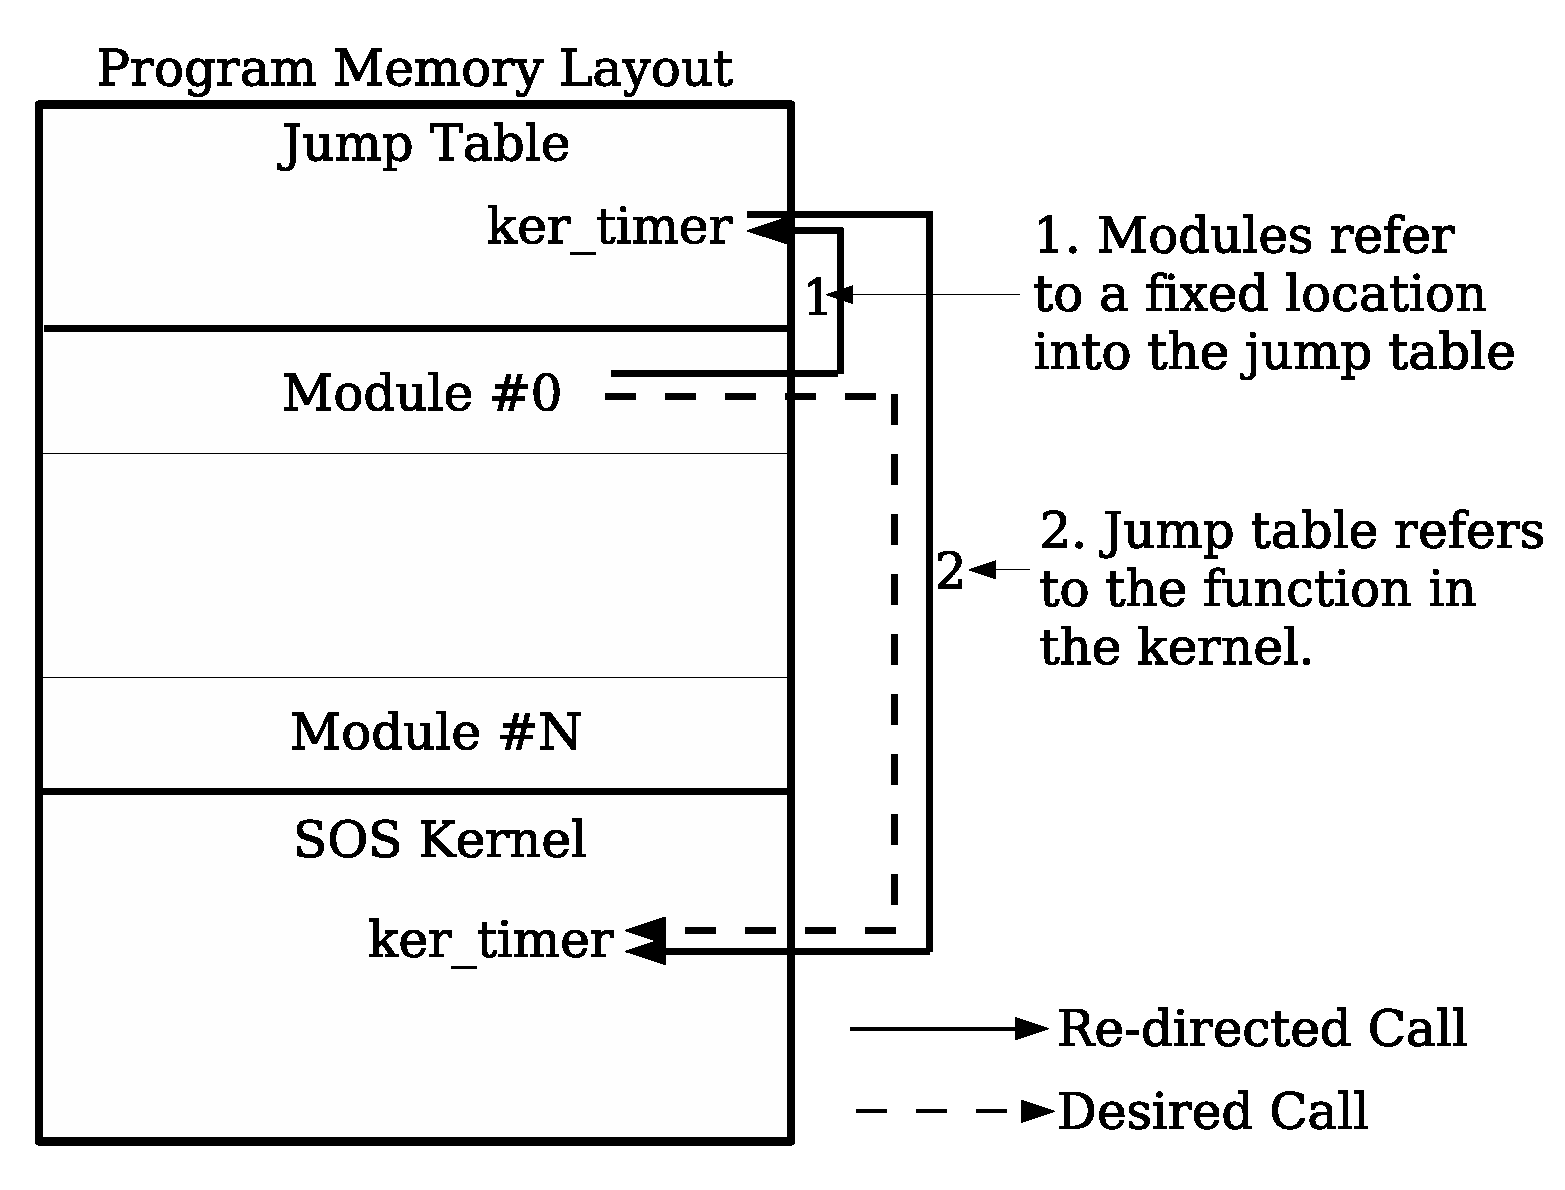
\includegraphics[height = 1.75in,
% %   keepaspectratio=true]{figures/jumptable.eps} 
% %   \caption{Jump Table for SOS Modules}
% %   \label{fig:sosjmptbl}
% % \end{figure}
% %----------------------------------------------------------
% \subsubsection{Message Passing}
% %
% The modules in SOS can communicate with other modules and the kernel
% through message passing.
% %
% SOS modules are implemented as message handlers as shown in
% Figure~\ref{fig:modinteract}.
% %
% The messages are annotated with the identity of the destination module
% and stored in a FIFO queue within the kernel.
% %
% The scheduler invokes a handler function in the destination module of
% a message.
% %
% During load time, the modules register the handler function with
% the kernel.
% %
% %All modules are required to implement a message handler.
% %
% The message handlers execute in the background context.
% %
% The background context comprises of operations that can only be
% interrupted by events occurring in the foreground context (for
% e.g. hardware interrupts).
% %
% %A module can invoke synchronous system calls in the kernel and
% %synchronous function calls in the other modules from a message
% %handler.
% %
% After a handler terminates, the execution control is transferred back
% to the scheduler.
% %
% SOS requires cooperative scheduling to share the processor between
% multiple executing modules.
% %
% %---------------------------------------------------------
% \subsubsection{Dynamic Memory Allocation}
% % 
% The SOS kernel supports dynamic memory allocation.
% % 
% Dynamic memory is used to store module state and to create messages to
% be dispatched to other modules. 
% % 
% Memory is allocated using a block-based first-fit scheme to minimize
% the overhead of the allocation process.
% %
% The size of the block is platform dependant and is 8 bytes for Mica2
% sensor node.
% % 
% Limited memory forces SOS kernel and user modules to share a common
% allocation heap; any static partitioning would be too conservative.
% % 
% % The dynamic memory is shared by the SOS kernel and the modules.
% % 
% The kernel therefore tracks ownership of memory blocks.
% % 
% A block's ownership can also be transferred, allowing
% % 
% buffers to pass easily through various modules in the system.
% 
% 
%====================================================================== 
% \subsection{System Components}
% % 
% Harbor's four components are shown in Figure~\ref{fig:sys_overview}.
% % 
% %% We first describe overall system operation.
% % 
% The system's input consists of raw user module binaries generated by a
% cross-compiler toolchain.
% % 
% The \emph{binary rewriter} is a desktop application that statically
% analyzes these binaries for potentially unsafe operations and inserts
% run-time checks to sandbox them.
% % 
% The sandboxed binary is then distributed to a network of sensor nodes.
% % 
% A \emph{verifier} running on each node verifies that incoming binaries
% are correctly sandboxed.
% % 
% Verified binaries admitted for execution interact closely
% with Harbor's run-time components, the \emph{memory map manager} and \emph{control flow
%   manager}.
% %
% \begin{figure}[htbp]
%   \centering
%   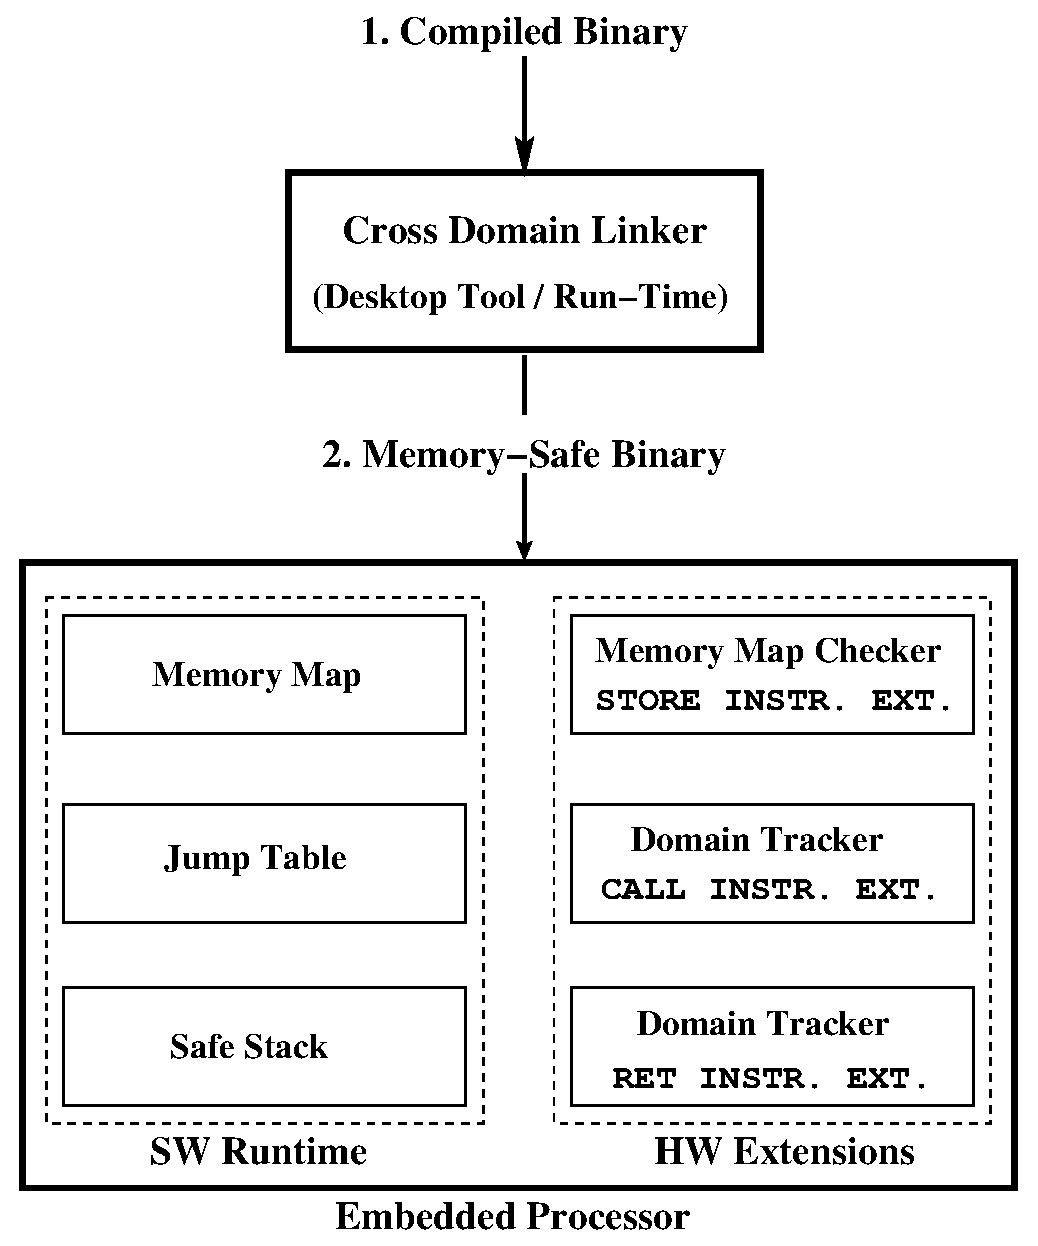
\includegraphics[height = 2.0in, keepaspectratio=true]{figures/sysoverview.eps} 
%   \caption{System Overview}
%   \label{fig:sys_overview}
% \end{figure}



%------------------------------------------------------------------
%\subsection{Summary}
%
This section positions Harbor in the category of fault isolation
techniques for
resource constrained microcontrollers.
% with limited address space.
%
Harbor isolation is more fine-grained than other approaches for sensor
networks.
%
The design of Harbor, though motivated by systems in the
desktop/server domains, introduces new techniques that address the
embedded domain's constraints.
%
%Finally, the brief overview of SOS presented in this section is
%essential to completely understand the implementation details.

%===========================================================================
% CONCLUSION
%===========================================================================
\section{Conclusion}
\label{sec:conclude}
%
In this paper, we have proposed a hardware software co-design approach for providing memory protection in tiny embedded processors.
%
Though we have implemented the protection technology for the AVR microcontroller, our general approach is applicable to other RISC architectures such as TI MSP or ARM.
%
Through a careful partitioning of the protection techniques, we have significantly improved performance by moving compute intensive operations into hardware.
%
Our hardware is very flexible, it can accommodate various configuration parameters.
%
The software library provides a standard programming interface.
%
Moreover, our approach does not modify the instruction set architecture of the processor; hence we do not need to modify the cross compiler.
%
These features ensure that our software library can be incorporated into existing projects with minimal modifications; a very practical benefit to the system developers.
%
We are still exploring the design space of possible protection architectures.
%
The resource utilization of our design can be further reduced by synthesizing hardware units that are pre-configured for a particular block size and number of protection domains.
%
An interesting area of future work is to explore software techniques such as virtual machines or type-safe languages  that can benefit from modest hardware extensions.
%
Software reliability is an emerging concern in the domain of tiny embedded processors.
%
Limited resources preclude the application of existing approaches used in desktop processors.
%
We believe that hardware software co-design techniques are a promising avenue to explore for creating robust software for tiny embedded processors. 


\footnotesize{
\bibliographystyle{abbrv}
\bibliography{ramthesis}
}

\end{document}
